%%%%%%%%%%%%%%%%%%%%%%%%%%%%%%%%%%%%%%%%%%%%%%%%%%%%%%
% A Beamer template for University of Wollongong     %
% Based on THU beamer theme                          %
% Author: Qiuyu Lu                                   %
% Date: July 2024                                    %
% LPPL Licensed.                                     %
%%%%%%%%%%%%%%%%%%%%%%%%%%%%%%%%%%%%%%%%%%%%%%%%%%%%%%
% Customized for Sharif University of Technology     %
%%%%%%%%%%%%%%%%%%%%%%%%%%%%%%%%%%%%%%%%%%%%%%%%%%%%%%


\documentclass[serif, aspectratio=169]{beamer}
\usepackage{pgfplots} % Required for plotting
\pgfplotsset{compat=1.17} % Compatibility level
%\documentclass[serif]{beamer}  % for 4:3 ratio
\usepackage[T1]{fontenc} 
\usepackage{fourier} % see "http://faq.ktug.org/wiki/uploads/MathFonts.pdf" for other options
\usepackage{hyperref}
\usepackage{latexsym,amsmath,xcolor,multicol,booktabs,calligra}
\usepackage{graphicx,pstricks,listings,stackengine}
\usepackage{lipsum}
\usepackage{array}    
\usepackage{soul} 

\author{Ali Sharifi-Zarchi}
\title{Machine Learning (CE 40477)}
\subtitle{Fall 2024}
\institute{
    CE Department \\
    Sharif University of Technology
}
%\date{\small \today}
% \usepackage{UoWstyle}
\usepackage{SUTstyle}

% defs
\def\cmd#1{\texttt{\color{red}\footnotesize $\backslash$#1}}
\def\env#1{\texttt{\color{blue}\footnotesize #1}}
\definecolor{deepblue}{rgb}{0,0,0.5}
\definecolor{deepred}{RGB}{153,0,0}
\definecolor{deepgreen}{rgb}{0,0.5,0}
\definecolor{halfgray}{gray}{0.55}

\lstset{
    basicstyle=\ttfamily\small,
    keywordstyle=\bfseries\color{deepblue},
    emphstyle=\ttfamily\color{deepred},    % Custom highlighting style
    stringstyle=\color{deepgreen},
    numbers=left,
    numberstyle=\small\color{halfgray},
    rulesepcolor=\color{red!20!green!20!blue!20},
    frame=shadowbox,
}


\begin{document}

\begin{frame}
    \titlepage
    \vspace*{-0.6cm}
    \begin{figure}[htpb]
        \begin{center}
            
\includegraphics[keepaspectratio, scale=0.25]{pic/sharif-main-logo.png}
        \end{center}
    \end{figure}
\end{frame}

\begin{frame}    
\tableofcontents[sectionstyle=show,
subsectionstyle=show/shaded/hide,
subsubsectionstyle=show/shaded/hide]
\end{frame}

\begin{frame}{Attention is All You Need!}
	\begin{figure}
		\centering
		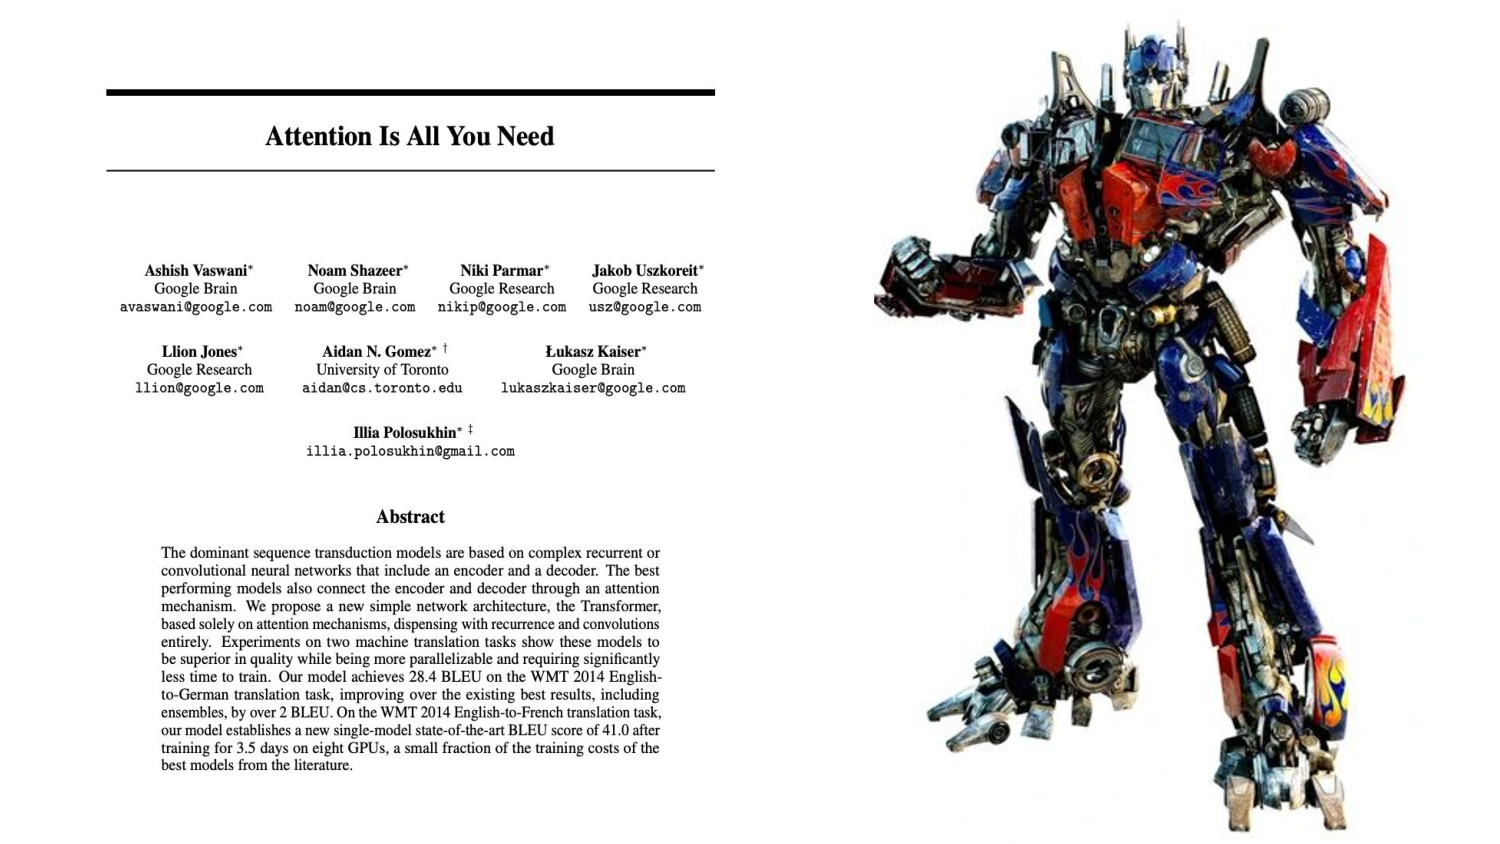
\includegraphics[width=0.9\linewidth]{pic/attention-is-all-you-need.pdf}
		\label{fig:attention-01}
	\end{figure}
	\begin{tikzpicture}[remember picture,overlay]
		\node[anchor=south west, xshift=0.09cm, yshift=0.3cm] at (current page.south west) {\tiny \href{https://arxiv.org/abs/1706.03762}{https://arxiv.org/abs/1706.03762}};
	\end{tikzpicture}
\end{frame}
\newpage

\begin{frame}{Attention: A Game-Changer in Natural Language Processing}
	\begin{itemize} 
		
		\item Imagine trying to read a book while your attention is scattered. You’d miss crucial details.
		\item Attention mechanism solve this problem in Neural Networks.
		\item This mechanism allows model to \textbf{“attend”} the most relevant information from the entire sequence.
		
	\end{itemize}
\end{frame}

\section{Contextualized Word Embeddings}

\begin{frame}{Limitations of Word2vec}
    \begin{itemize} 
    
        \item One vector for each word type
        
        \item Word2vec has challenges in polysemous words, e.g. \texttt{Light}
       % {شیر جنگل، شیر خوراکی و شیر آب}
        \item Words don’t appear in isolation. The word use (e.g., syntax and semantics) depends on its context.
        
        \item \textbf{Why not learn the representations for each word in its context?}

        \end{itemize}
\end{frame}


\begin{frame}{Contextualized Word Embeddings}
		
	\begin{figure}
		\centering
		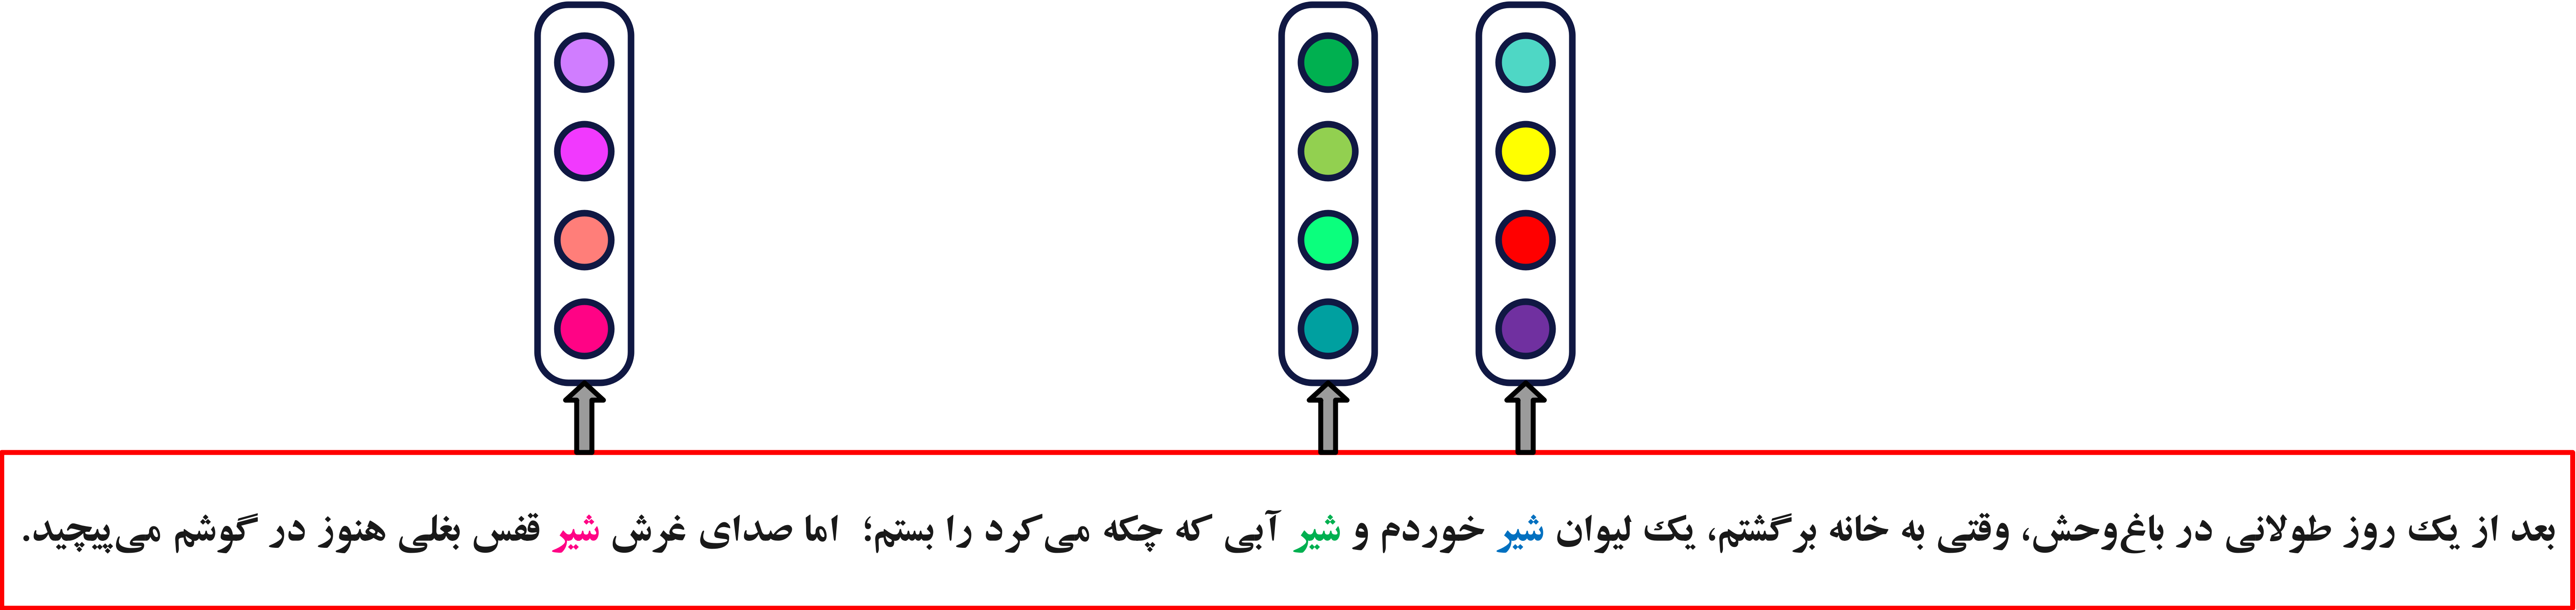
\includegraphics[width=0.95\textwidth]{pic/example-2.png}
		\label{fig:Contextualized-word-embedding-1}
	\end{figure}
	\vspace{-5pt}
	\begin{figure}
		\centering
		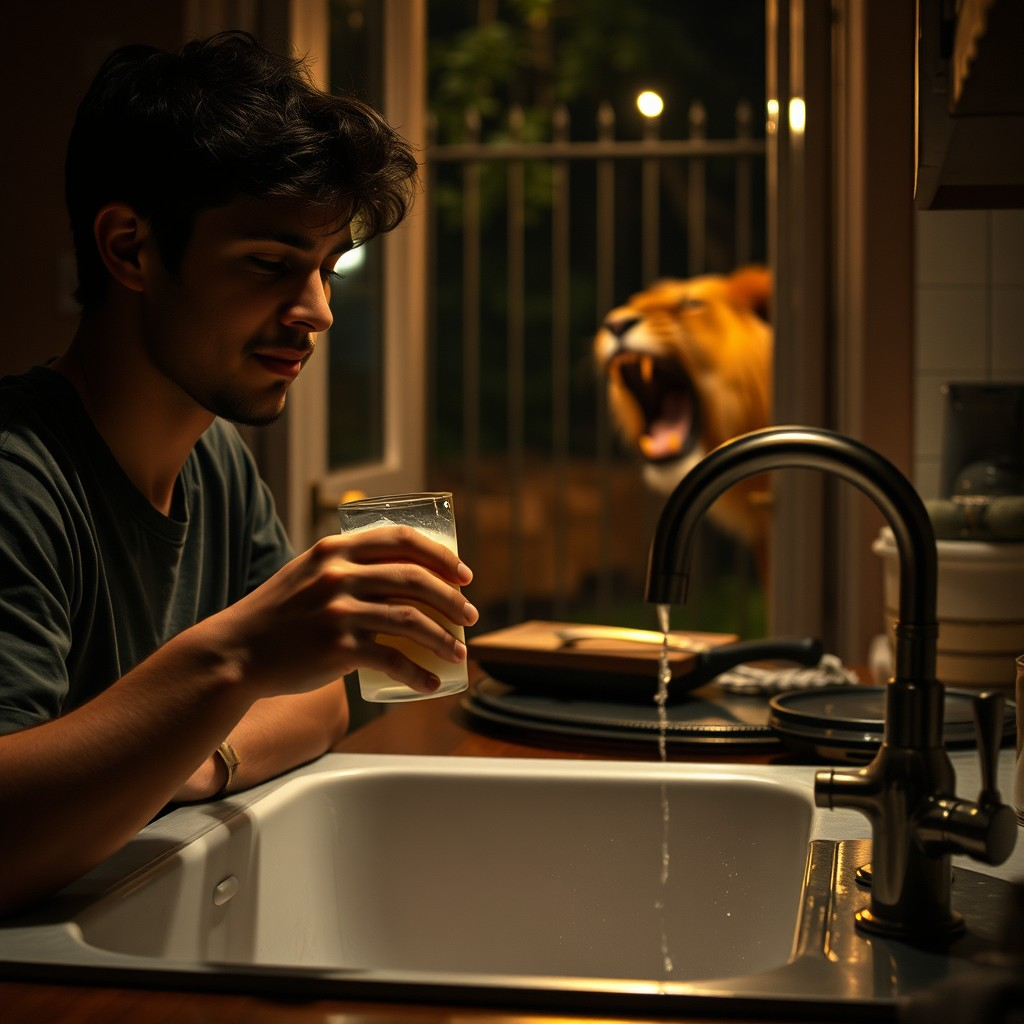
\includegraphics[width=0.27\textwidth]{pic/Flux-1.png}
		\label{fig:Contextualized-word-embedding-1}
	\end{figure}
	
	\vfill
	\begin{tikzpicture}[remember picture,overlay]
		\node[anchor=south west, xshift=0.15cm, yshift=0.22cm] at (current page.south west) {
			\tiny Figure generated by Flux.1
		};
	\end{tikzpicture}
	
\end{frame}


\begin{frame}{Contextualized Word Embeddings}
	Compute contextual vector:
	\[
	\mathbf{c_k} = f(w_k \mid w_1, w_2, \dots, w_n) \in \mathbb{R}^d
	\]
	\noindent Examples:
	\vspace{-5pt}
	\[
	f(\textcolor{green}{light} \mid \text{Please turn off the }\overbrace{\textcolor{green}{light}}^{
\includegraphics[height=3em]{pic/1.png}}\text{.})
	\]
	\[\neq\]
	\[
	f(\textcolor{orange}{light} \mid \text{This box is very }\underbrace{\textcolor{orange}{light}}_{
\includegraphics[height=4em]{pic/Flux-light-weight.jpeg}}\text{ to carry.})
	\]
	\textbf{How do we implement the context function $f$?}
	\vspace{5pt}
\end{frame}

\section{Recurrent Neural Networks}

\begin{frame}{Recurrent Neural Networks}
	\begin{itemize}
		\item To process each word, we need to remember the previous words.
		\item How do we create this memory? By maintaining a \textbf{hidden state}.
		\item Each hidden state captures information about:
		\begin{itemize}
			\item Current word
			\item All previous words in the sequence
		\end{itemize}
	\end{itemize}
	
	%    \begin{equation*}
		%        h_t = f(W_{hh}h_{t-1} + W_{xh}x_t + b)
		%    \end{equation*}
	
	\begin{figure}
		\centering
		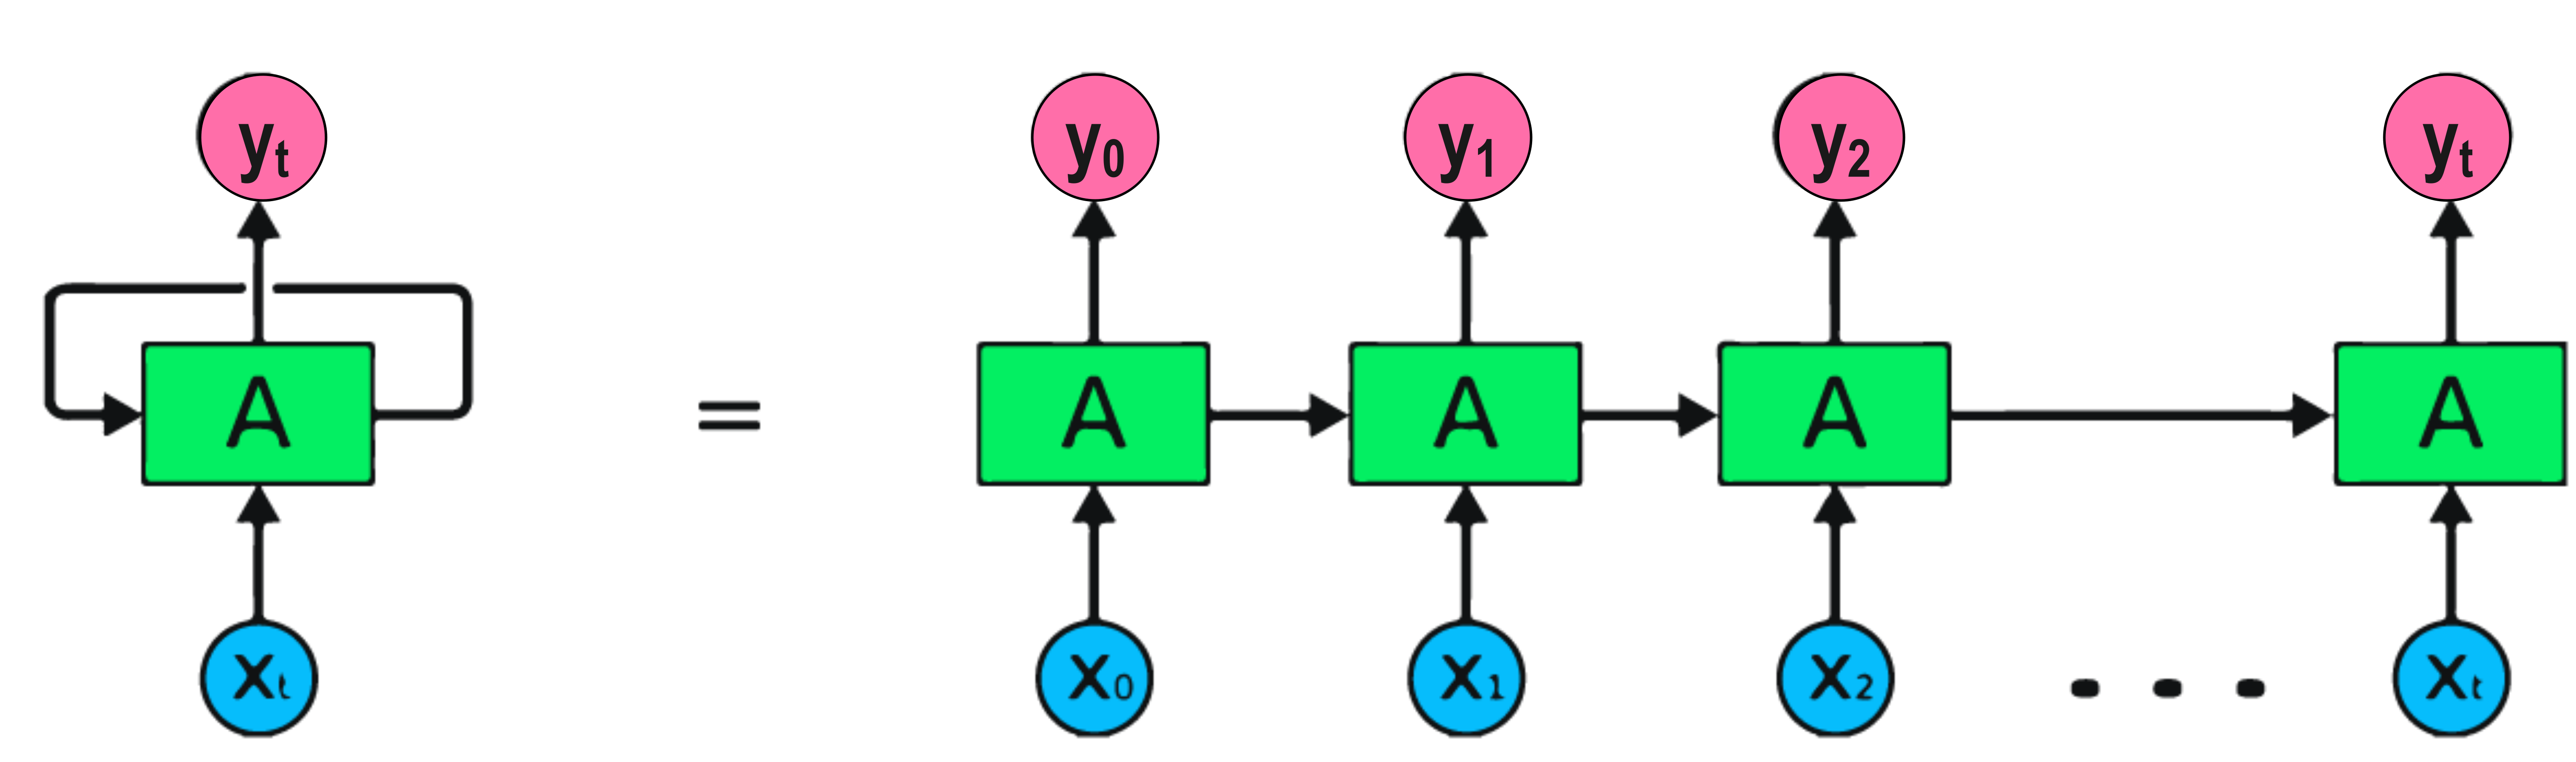
\includegraphics[width=0.6\textwidth]{pic/image-RNN.png}
		\label{fig:image-RNN}
	\end{figure}
	
	\begin{center}
		where $h_t$ serves as contextualized representation, containing memory of previous words.
	\end{center}
	
	\vfill
	\begin{tikzpicture}[remember picture,overlay]
		\node[anchor=south west, xshift=0.15cm, yshift=0.22cm] at (current page.south west) {
			\tiny Figure adapted from Abid Ali Awan. What are Recurrent Neural Networks (RNN), DataCamp
		};
	\end{tikzpicture}
	
	
\end{frame}


\begin{frame}{RNN's Hidden State Update}
    \begin{itemize}
        \item Process sequences by maintaining a hidden state.
        \item Update state sequentially: $h_t = f_W(h_{t-1}, x_t)$
        \item This recurrence formula is applied at each time step to process a sequence of vectors x.
        \item The same function and the same set of parameters are used for each word.
        
    \end{itemize}
     \begin{figure}
         \centering
         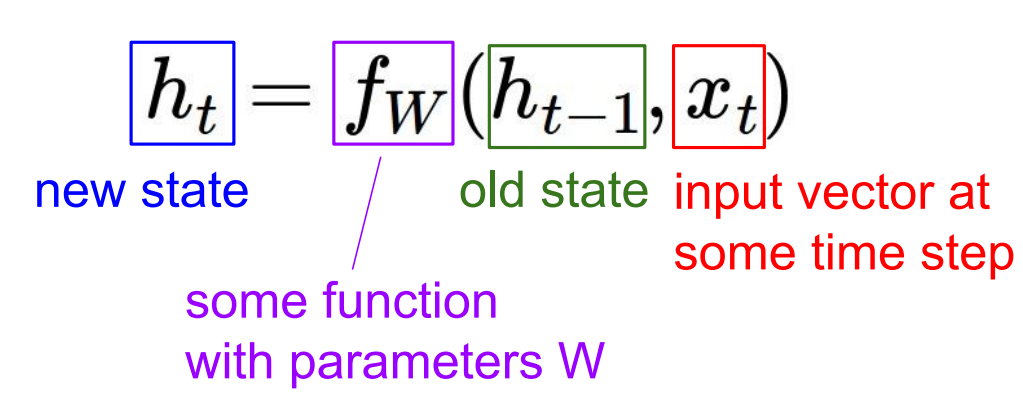
\includegraphics[width=0.4\textwidth]{pic/RNN-2.png}
     \end{figure}
\end{frame}

\begin{frame}{RNN Output Generation}
	\begin{itemize}
		\item After updating the hidden state, RNN generates outputs at each time step.
		\item The output \( y_t \) is typically computed as a function of the current hidden state \( h_t \), often passed through a layer (like a softmax layer) for classification or regression tasks.
	\end{itemize}
	\begin{figure}
		\centering
		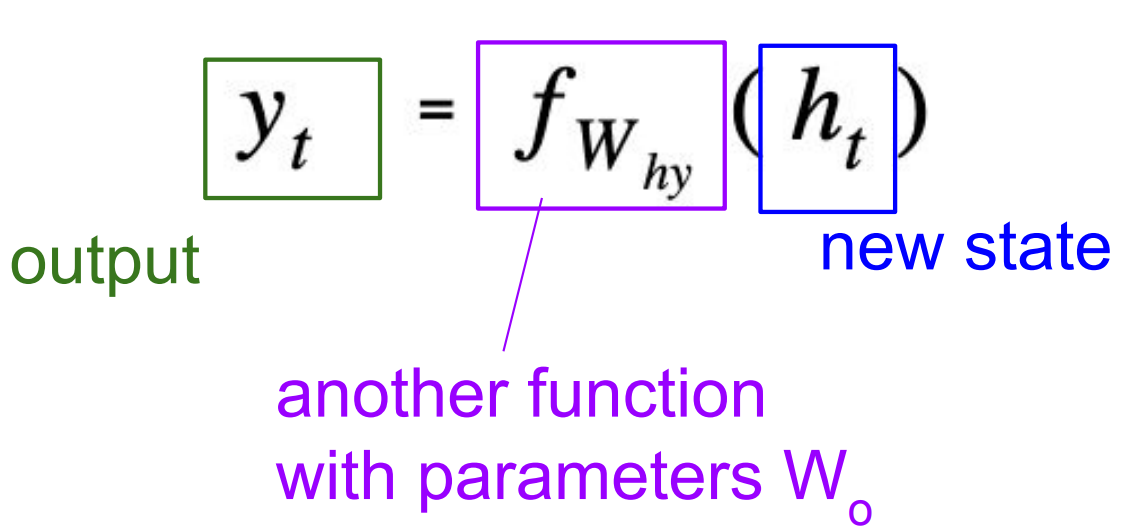
\includegraphics[width=0.4\textwidth]{pic/RNN-out.png}
	\end{figure}
\end{frame}

\begin{frame}{(Vanilla) Recurrent Neural Network}
	\begin{itemize}
		\item The state of the RNN consists of a single hidden vector \( h_t \), which updates as new inputs are processed.
	\end{itemize}
	\vspace{-35pt}
	\begin{figure}
		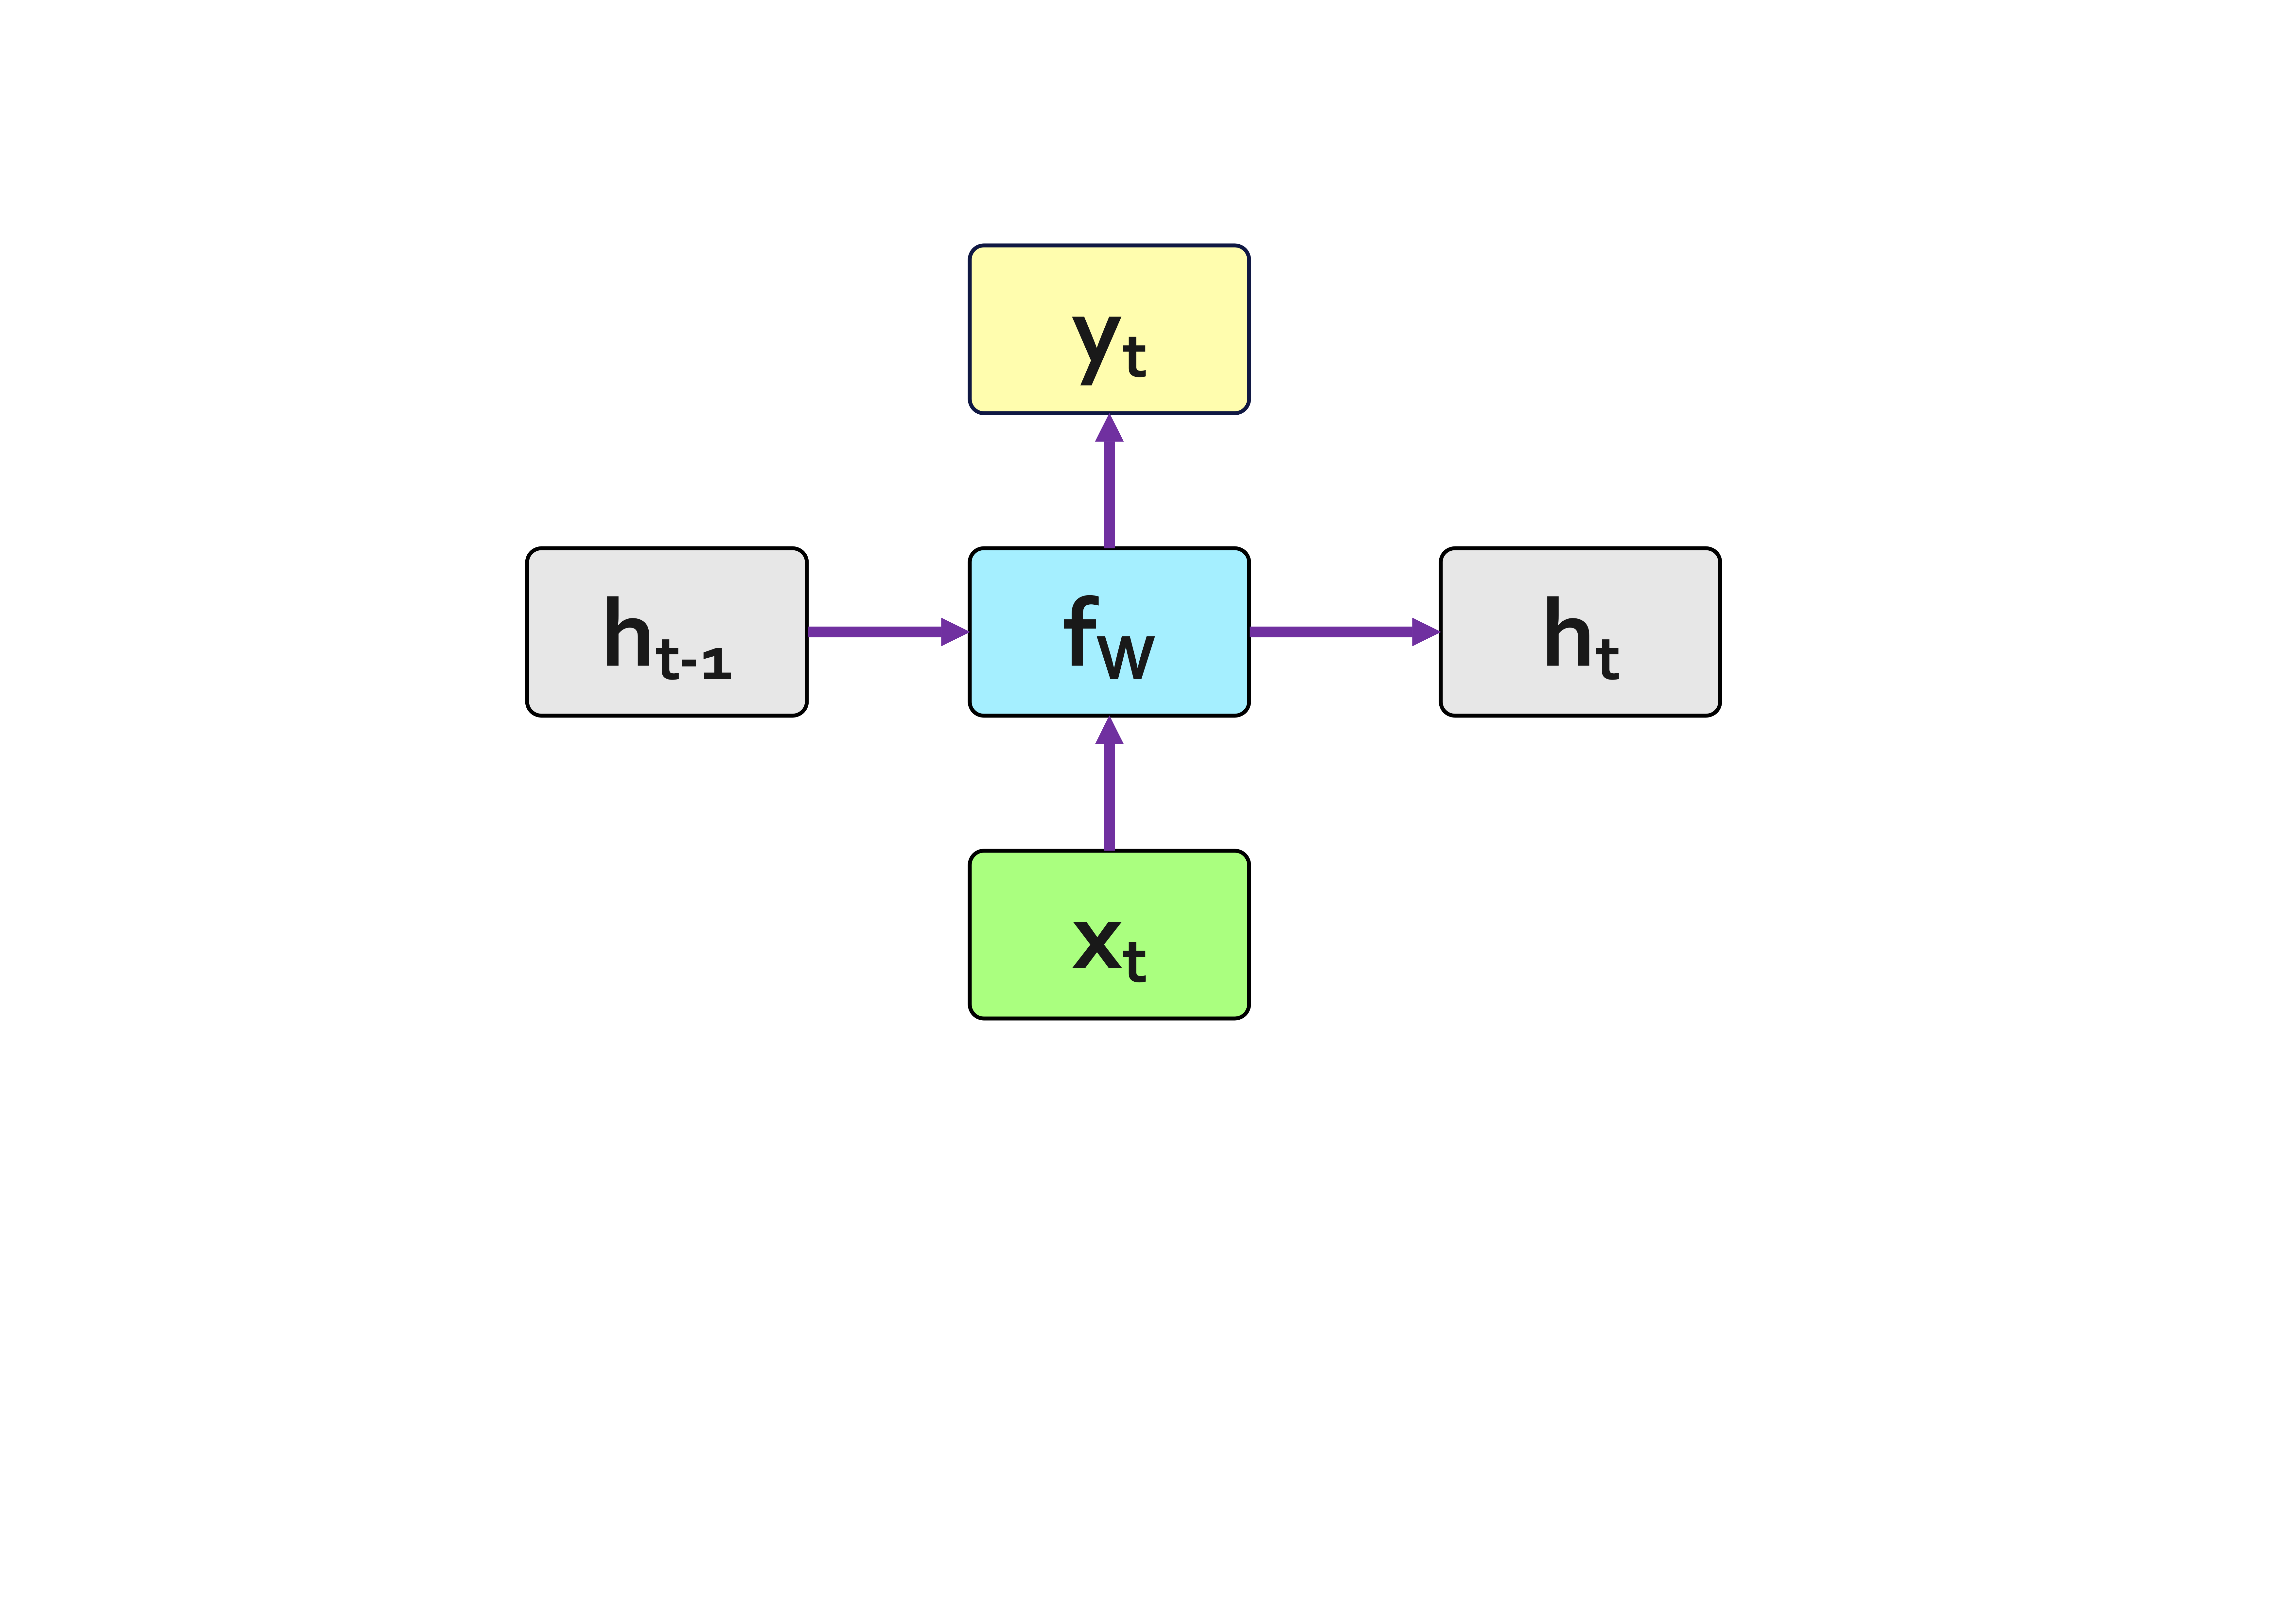
\includegraphics[width=0.7\textwidth]{pic/RNN-final.png}
		\caption{RNN hidden state update at time \( t \), where \( h_t \) represents the current context.}
	\end{figure}
	\vspace{-100pt}
	\begin{align*}
		h_t &= f_W(h_{t-1}, x_t) \\ 
		\downarrow \\
		h_t &= f(W_{hh} h_{t-1} + W_{xh} x_t + b) \\ 
		y_t &= W_{hy} h_t
	\end{align*}
\end{frame}

\begin{frame}{Basic Numerical Example of RNN - Hidden State Update (Part 1)}
	\begin{itemize}
		\item Consider a simple RNN with the following parameters:
		\begin{itemize}
			\item Input \( x_t = \begin{bmatrix} 1 \\ 0 \end{bmatrix} \)
			\item Previous hidden state \( h_{t-1} = \begin{bmatrix} 0.5 \\ -0.5 \end{bmatrix} \)
			\item Weight matrices: \[
			W_{hh} = \begin{bmatrix} 0.1 & 0.2 \\ -0.1 & 0.3 \end{bmatrix}, 
			W_{xh} = \begin{bmatrix} 0.4 & 0.5 \\ 0.6 & 0.7 \end{bmatrix}
			\]
			\item Bias vector \( b = \begin{bmatrix} 0.1 \\ 0.2 \end{bmatrix} \)
		\end{itemize}
		\item The RNN updates its hidden state using the equation:
		\vspace{-5pt}
		\[
		h_t = W_{hh} h_{t-1} + W_{xh} x_t + b
		\]
	\end{itemize}
	\vspace{-12pt}
	\begin{align*}
		h_t &= \begin{bmatrix} 0.1 & 0.2 \\ -0.1 & 0.3 \end{bmatrix} \begin{bmatrix} 0.5 \\ -0.5 \end{bmatrix} + \begin{bmatrix} 0.4 & 0.5 \\ 0.6 & 0.7 \end{bmatrix} \begin{bmatrix} 1 \\ 0 \end{bmatrix} + \begin{bmatrix} 0.1 \\ 0.2 \end{bmatrix}
	\end{align*}
\end{frame}

\begin{frame}{Basic Numerical Example of RNN - Hidden State Update (Part 2)}
	\begin{itemize}
		\item Continuing from the previous slide, the calculation after adding the bias term is:
	\end{itemize}
	\begin{align*}
		h_t &= \begin{bmatrix} 0.05 - 0.1 \\ -0.05 - 0.15 \end{bmatrix} + \begin{bmatrix} 0.4 \\ 0.6 \end{bmatrix} + \begin{bmatrix} 0.1 \\ 0.2 \end{bmatrix} \\
		h_t &= \begin{bmatrix} 0.45 \\ 0.6 \end{bmatrix}
	\end{align*}
	\vspace{-10pt}
	The hidden state is then passed through the activation function (tanh):
	\begin{align*}
		h_t &= f\left(\begin{bmatrix} 0.45 \\ 0.6 \end{bmatrix}\right) \\
		h_t &= \begin{bmatrix} \tanh(0.45) \\ \tanh(0.6) \end{bmatrix}
	\end{align*}
\end{frame}

\begin{frame}{Basic Numerical Example of RNN - Output Computation}
	\begin{itemize}
		\item Continuing from the previous slide, the updated hidden state is:
		\[
		h_t = f\left(\begin{bmatrix} 0.45 \\ 0.6 \end{bmatrix}\right)
		\]
		\item The output \( y_t \) is computed as:
		\[
		y_t = W_{hy} h_t
		\]
	\end{itemize}
	\vspace{-15pt}
	\begin{align*}
		y_t &= \begin{bmatrix} 0.8 & 0.9 \end{bmatrix} \begin{bmatrix} \tanh(0.45) \\ \tanh(0.6) \end{bmatrix} \\
		y_t &= \begin{bmatrix} 0.8 \cdot 0.4228 + 0.9 \cdot 0.5370 \end{bmatrix} \\
		y_t &= \begin{bmatrix} 0.3382 + 0.4833 \end{bmatrix} \\
		y_t &= \begin{bmatrix} 0.8215 \end{bmatrix}
	\end{align*}
\end{frame}

\begin{frame}{Challenges of RNNs}
		While improved versions of vanilla RNNs attempt to resolve some issues, in many cases they still struggle with:
		\begin{itemize}
			\item Long-term dependencies
			\item Vanishing/exploding gradients
			\item Sequential computation (can't parallelize)
		\end{itemize}
\end{frame}

\begin{frame}{Challenges of RNNs}
		RNNs face challenges in retaining information over long sequences, such as when pronouns refer to distant words in the sequence.
		\begin{figure}
			\centering
			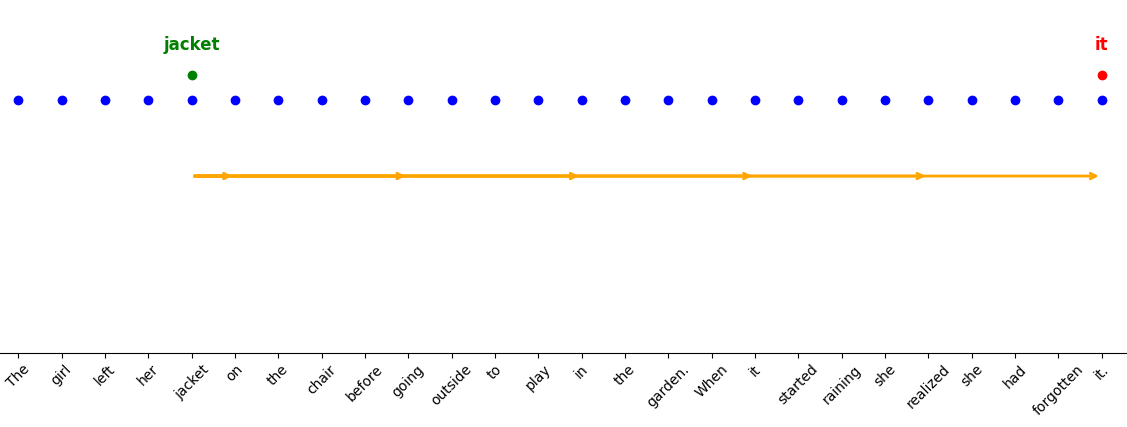
\includegraphics[width=0.99\textwidth]{pic/RNN-challenges.png}
			\label{fig:RNN-challenges}
		\end{figure}
		\textbf{So, what solution do we have?}
\end{frame}

\section{Attention Mechanism}

\begin{frame}{Why Attention?}
	\begin{itemize}
		\item Enhances the model's ability to focus on relevant parts of the input.
		\item Can compute relationships between inputs regardless of their position.
		\item Inspired by human visual attention.
		\item \textbf{Key Idea}
		\begin{itemize}
			\item Let the model learn which parts of the input are important for each output.
		\end{itemize}
	\end{itemize}
\end{frame}

\begin{frame}{Why Attention?}
    \begin{figure}
        \centering
        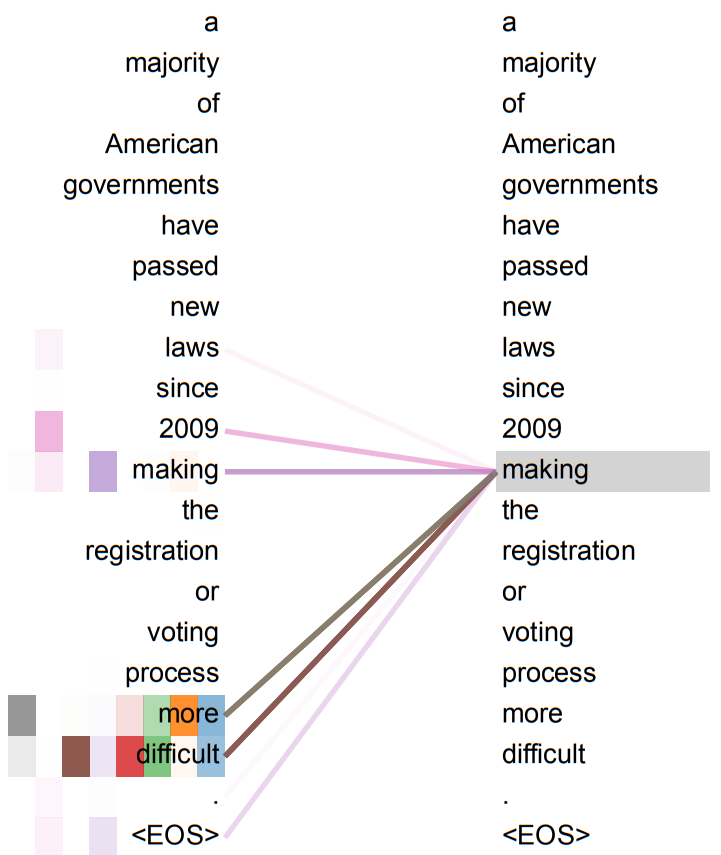
\includegraphics[width=0.415\textwidth]{pic/Attention-1.png}
        \label{fig:Attention-1}
    \end{figure}
    
    	\vfill
    \begin{tikzpicture}[remember picture,overlay]
    	\node[anchor=south west, xshift=0.15cm, yshift=0.22cm] at (current page.south west) {
    		\tiny Figure adapted from Ashish Vaswani et al. Attention is All You Need paper
    	};
    \end{tikzpicture}
\end{frame}

\begin{frame}{Attention as a Soft, Averaging Lookup Table}
\begin{figure}[!htb]
    \centering
    \begin{minipage}{0.4\textwidth}
        \centering
        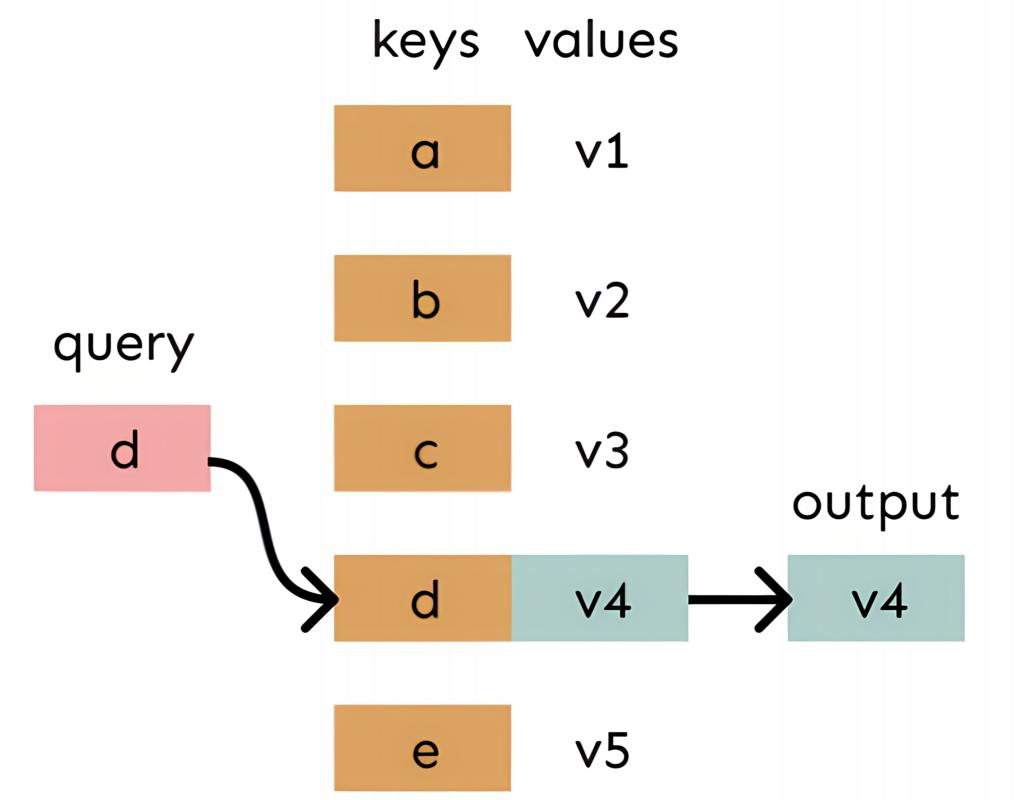
\includegraphics[width=\textwidth]{pic/attention-3.png}
        In a \textcolor{orange}{lookup table}, we have a table of keys that map to values. The query matches one of the keys, returning its value.
        \label{fig:attention-4}
        
    \end{minipage}%
    \hfill
    {\vrule width 1pt}
    \hfill
    \begin{minipage}{0.48\textwidth}
        \centering
        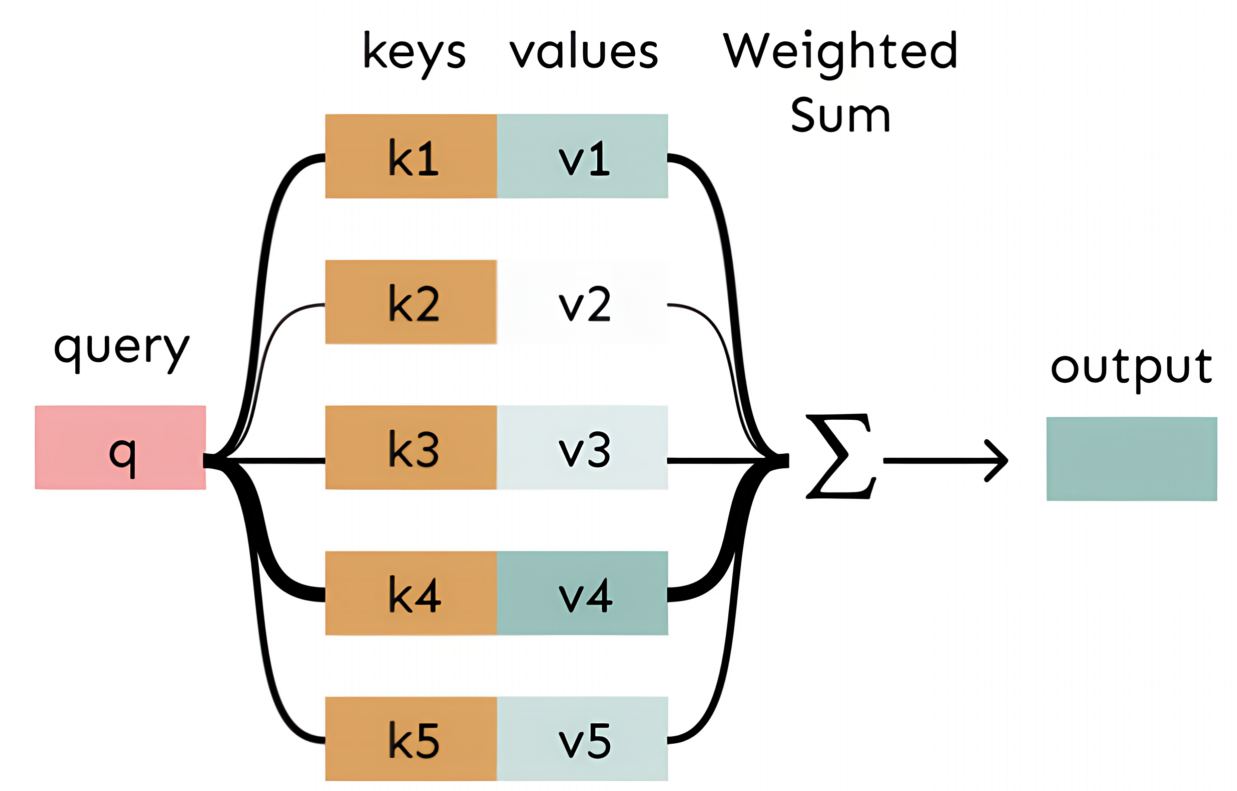
\includegraphics[width=\textwidth]{pic/attention-4.png}
                In the \textcolor{green}{attention}, the query matches all keys softly, to a weight between 0 and 1. The keys' values are multiplied and summed by the weights.
        \label{fig:attention-3}
    \end{minipage}
\end{figure}
\vfill
\begin{tikzpicture}[remember picture,overlay]
	\node[anchor=south west, xshift=0.15cm, yshift=0.22cm] at (current page.south west) {
		\tiny Figure adapted from Chris Manning, Lecture Slides, Stanford University
	};
\end{tikzpicture}
\end{frame}

\begin{frame}{Attention Mechanism}
	\begin{itemize}
		\item An attention function maps a query and a set of key-value pairs to an output.
		\item The query, keys, values, and the output are represented as vectors.
		\item Components of the Attention Mechanism are:
		    \begin{itemize}
			\item Query (Q): What we're looking for
			\item Key (K): What we match against
			\item Value (V): What we retrieve
			\end{itemize}
		\item The most common attention function is \textbf{Scaled Dot Product Attention}, which will be described in the following slides.
	\end{itemize}
\end{frame}
%    \begin{equation*}
%        \text{Attention}(Q, K, V) = \text{softmax}\left(\frac{QK^T}{\sqrt{d_k}}\right)V
%    \end{equation*}
%    \begin{itemize}
%        \item $d_k$: dimension of keys (scaling factor)
%        \item Softmax converts scores to probabilities
%    \end{itemize}

\begin{frame}{Scaled Dot-Product Attention}
	\vspace{-5pt}
	\begin{center}
		     \hspace{14pt}\textbf{Output}
	\end{center}
	\vspace{-7pt}
	\begin{figure}
		\centering
		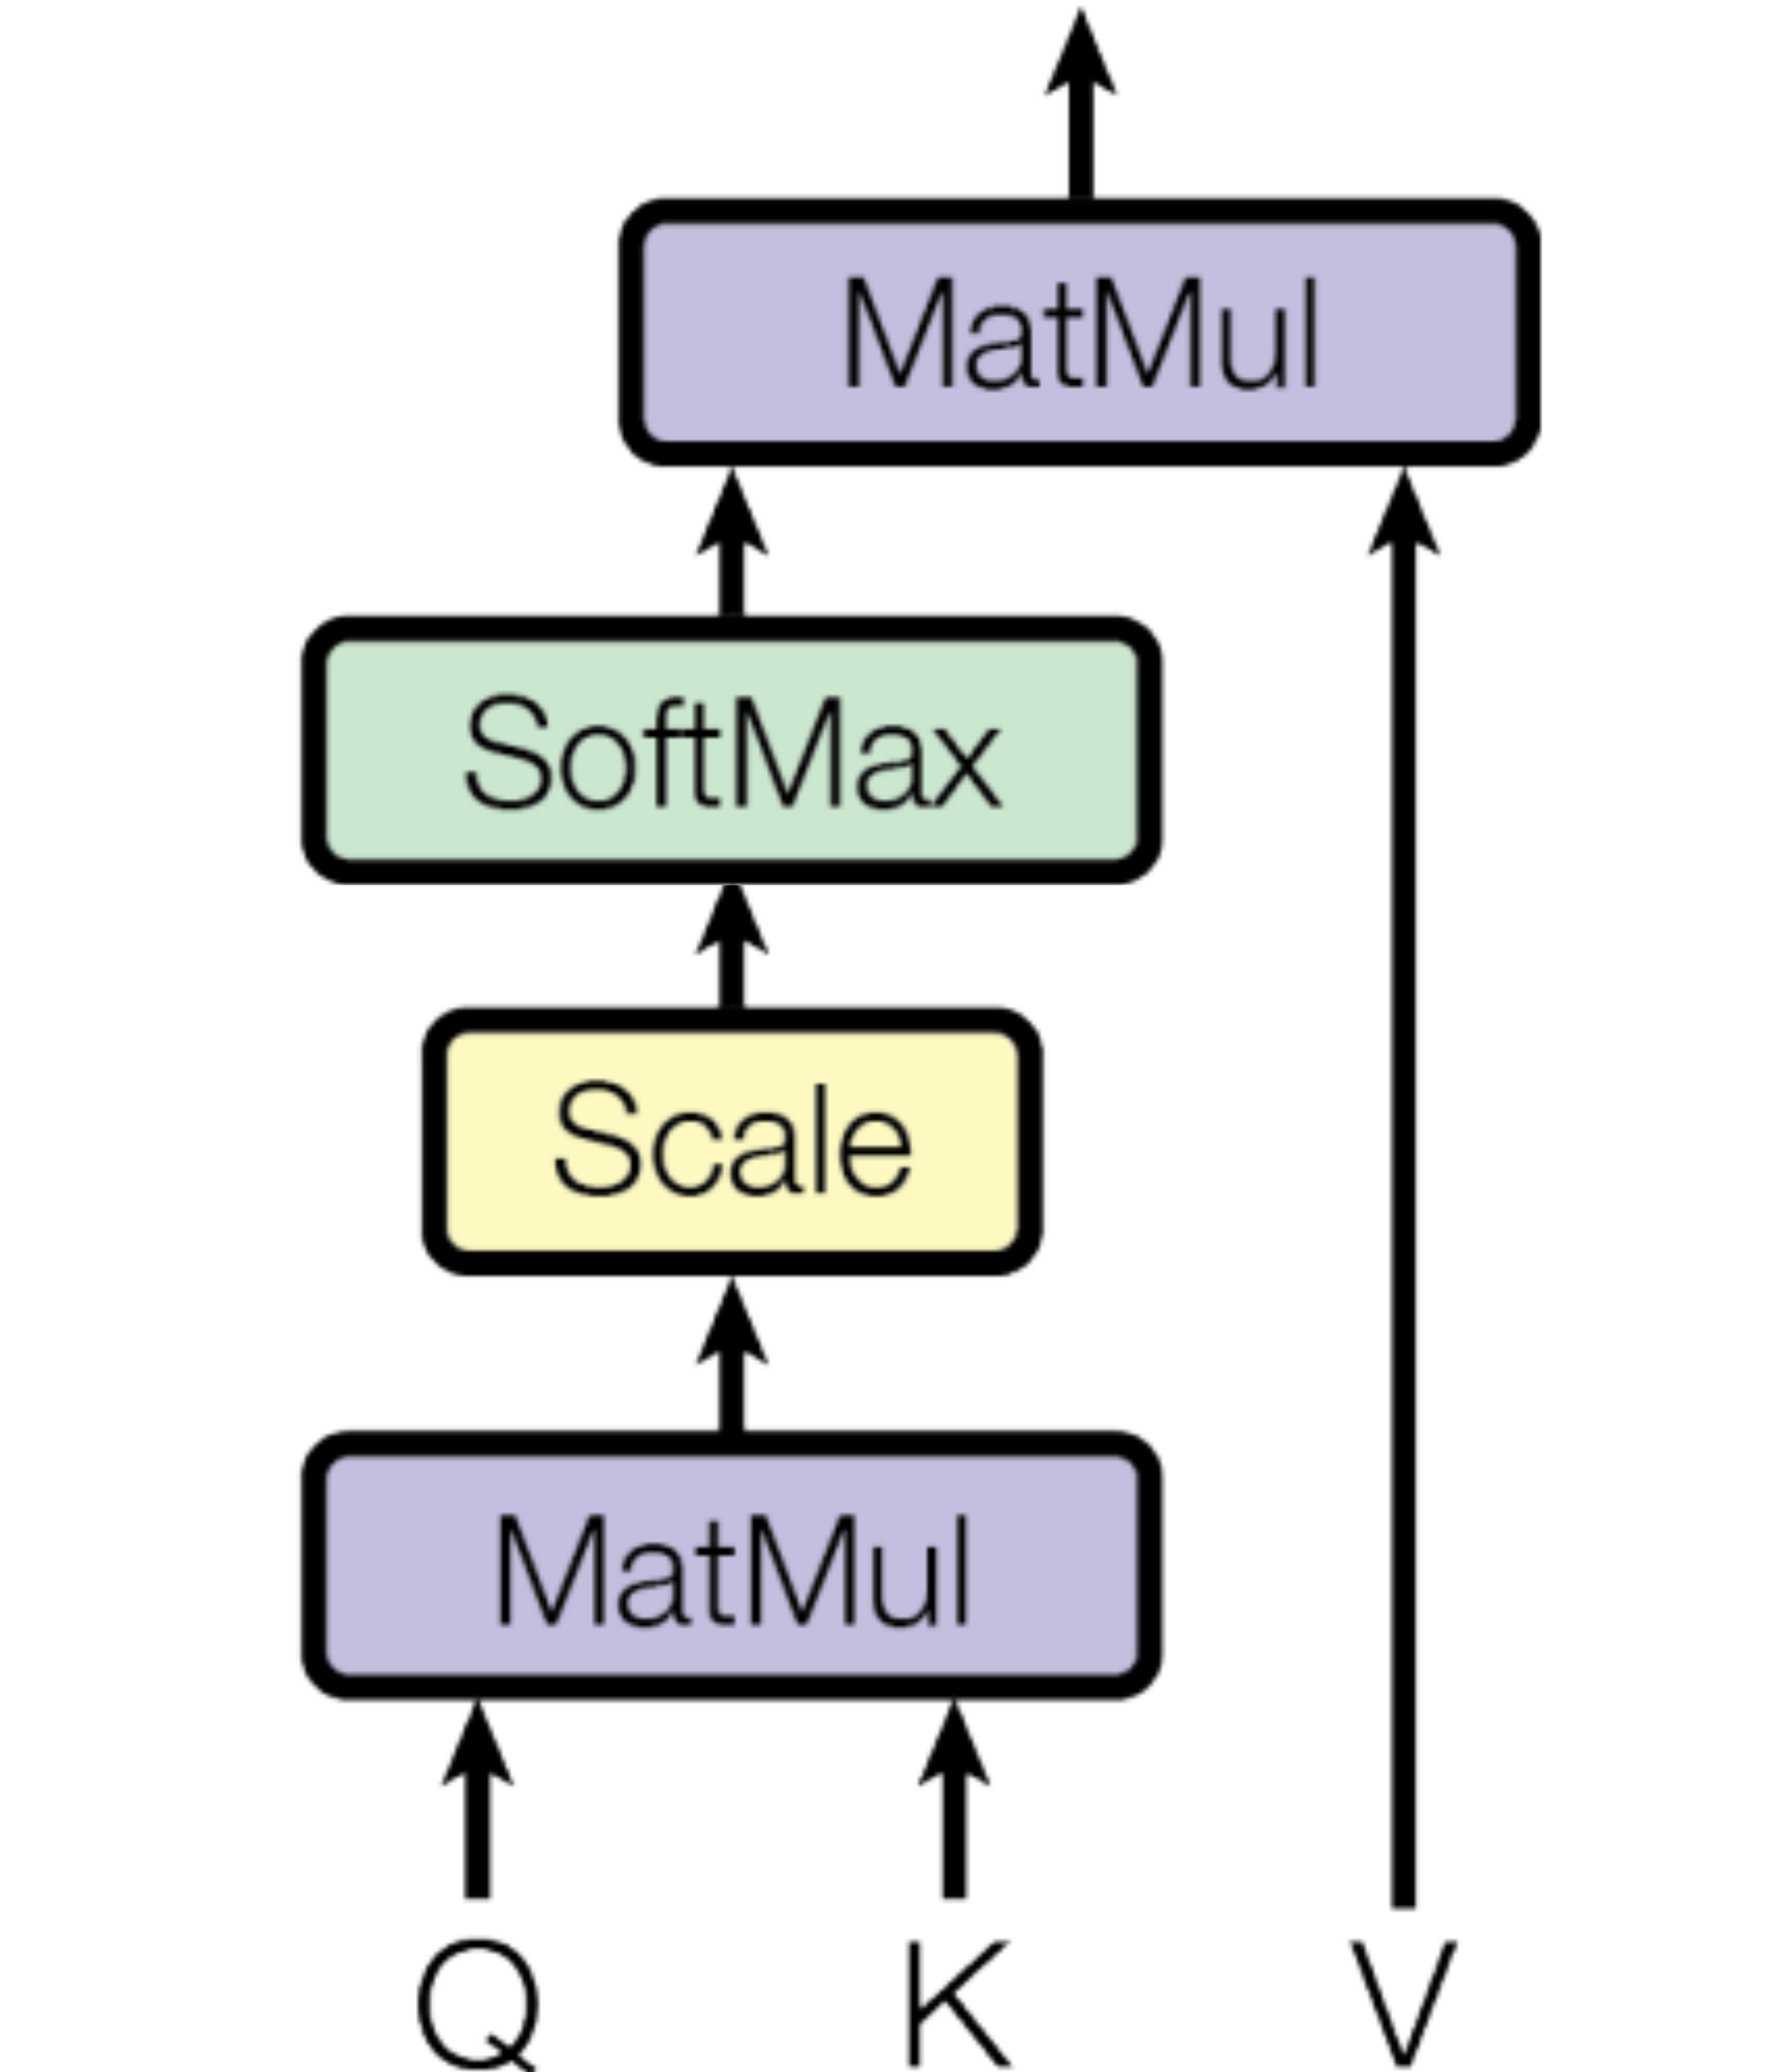
\includegraphics[width=0.3\textwidth]{pic/Attention-s-1.png}
		\label{fig:attention-2}
	\end{figure}
	\vspace{-10pt}
	
	%		\item Scaled dot-product attention function:
	\[
	\text{Attention}(Q, K, V) = \text{softmax}\left(\frac{QK^T}{\sqrt{d_k}}\right)V
	\]
	\vspace{4pt}
	\vfill
	\begin{tikzpicture}[remember picture,overlay]
		\node[anchor=south west, xshift=0.15cm, yshift=0.22cm] at (current page.south west) {
			\tiny Figure adapted from Ashish Vaswani et al. Attention is All You Need paper
		};
	\end{tikzpicture}
\end{frame}

\begin{frame}{Scaled Dot-Product Attention}
	\begin{equation*}
		\text{Attention}(Q, K, V) = \text{softmax}\left(\frac{QK^T}{\sqrt{d_k}}\right)V
	\end{equation*}
	\begin{itemize}
		\item The query and keys are in dimension $d_k$.
		\item Dot products of the query with all keys are computed, divided by $\sqrt{d_k}$
		\item The softmax function is applied to convert scores to probabilities (get attention distribution).
	\end{itemize}
	
\end{frame}

\begin{frame}{Scaling Factor in Attention (Part 1)}
	\begin{itemize}
		\item The attention function computes the dot product between the query and key. 
		\item For \textbf{large $d_k$}, the dot products can become very large, which \textbf{pushes the softmax function} into regions where it has \textbf{extremely small gradients}, making the model less effective at learning.
		\item To address this, the dot product is scaled by $\frac{1}{\sqrt{d_k}}$, ensuring softmax operates in a stable range.
	\end{itemize}
\end{frame}

\begin{frame}{Scaling Factor in Attention (Part 2)}
	\begin{itemize}
		\item Scaling improves training stability, especially for large $d_k$ values.
		\item This adjustment avoids softmax saturation and enhances model performance.
	\end{itemize}
\end{frame}

\begin{frame}{General Attention Layer}
	\begin{columns}
		
		\column{0.42\textwidth}
		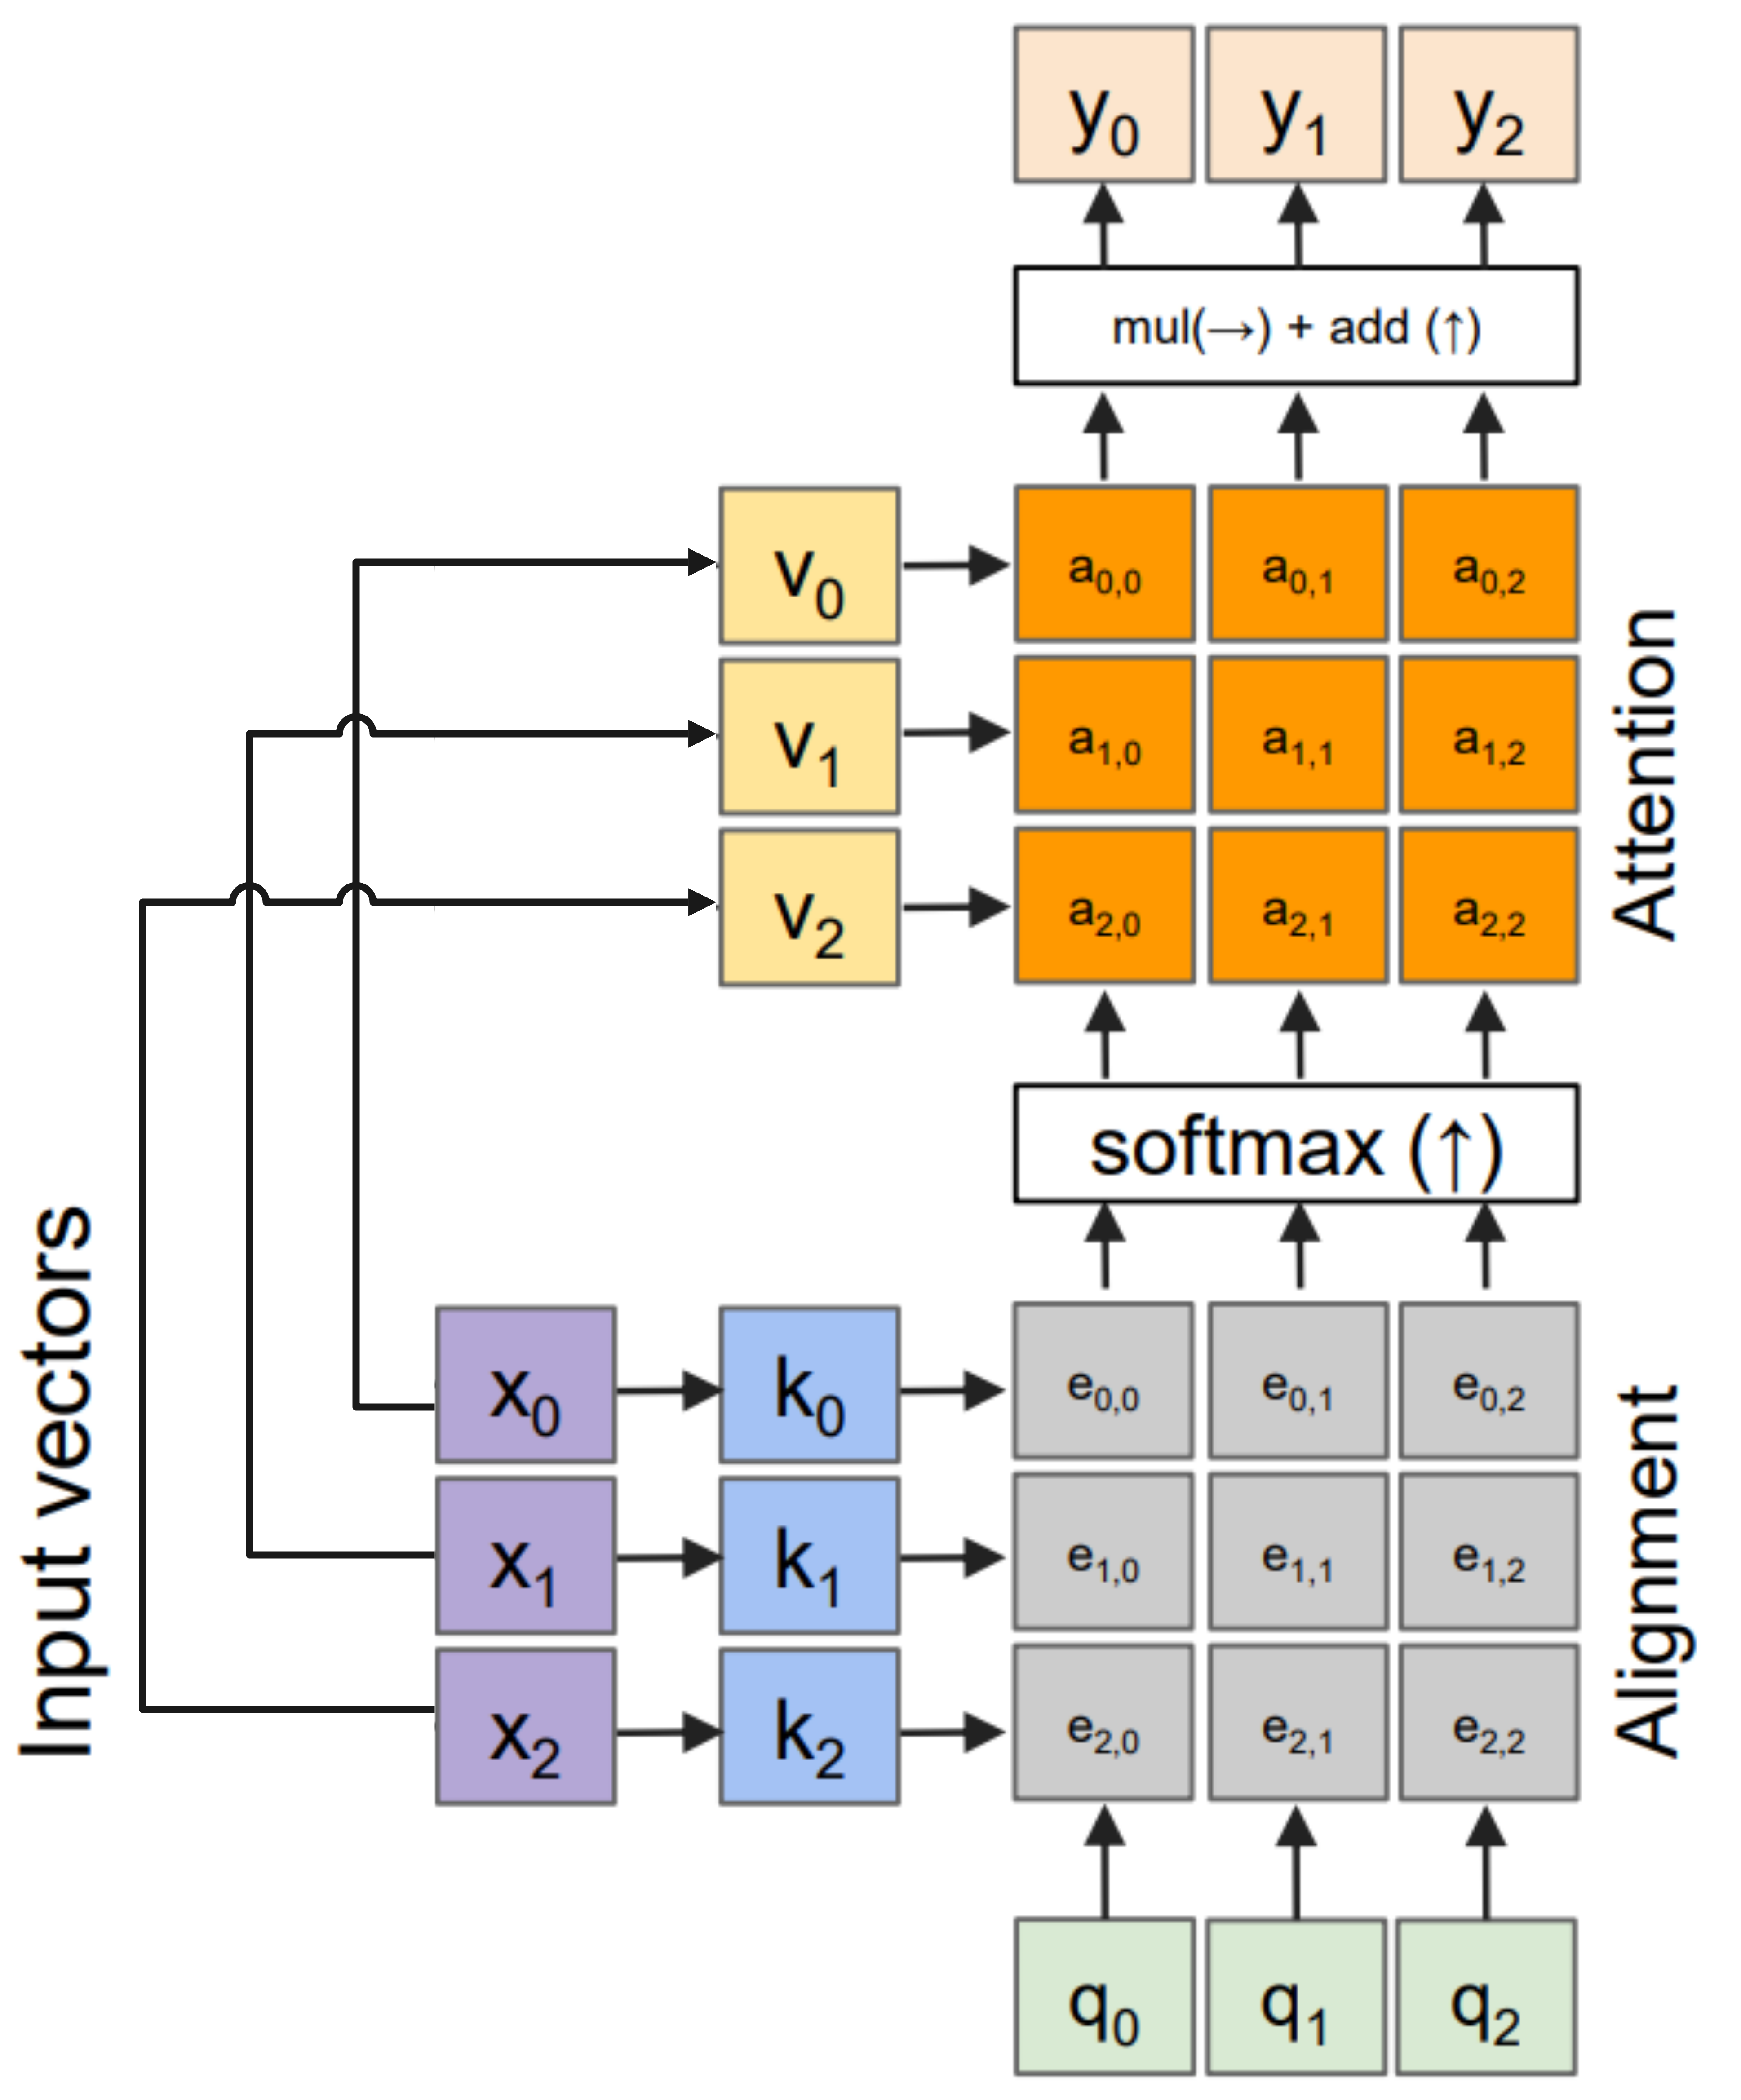
\includegraphics[width=0.95\textwidth]{pic/General-Attention-Layer-1.png}
		
		\column{0.58\textwidth}
		\textbf{Outputs:} \\
		Context vectors: $\mathbf{y}$ (\textit{shape: } $D_v$) \\[1em]
		
		\textbf{Operations:}
		\begin{itemize}
			\item Key vectors: $\mathbf{k} = W_k^T \mathbf{x}$
			\item Value vectors: $\mathbf{v} = W_v^T \mathbf{x}$
			\item \textbf{Alignment}: $e_{i,j} = \frac{\mathbf{q}_j \cdot \mathbf{k}_i}{\sqrt{D_k}}$
			\item \textbf{Attention}: $\mathbf{a} = \texttt{softmax}(\mathbf{e})$
			\item Output: $y_j = \sum_i a_{i,j} \mathbf{v}_i$
		\end{itemize}
		
		\textbf{Inputs:}
		\begin{itemize}
			\item Input vectors: $\mathbf{x}$ (\textit{shape: } $N \times D$)
			\item Queries: $\mathbf{q}$ (\textit{shape: } $M \times D_k$)
		\end{itemize}
	\end{columns}
\vspace{5pt}
\vfill
\begin{tikzpicture}[remember picture,overlay]
	\node[anchor=south west, xshift=0.15cm, yshift=0.22cm] at (current page.south west) {
		\tiny Figure adapted from Fei-Fei Li, Jiajun Wu, and Ruohan Gao Lecture Slides, Stanford University
	};
\end{tikzpicture}
\end{frame}

\begin{frame}{Self-Attention Layer}
		\begin{columns}
			% Left column: Image
			\begin{column}{0.25\textwidth}
				\centering
				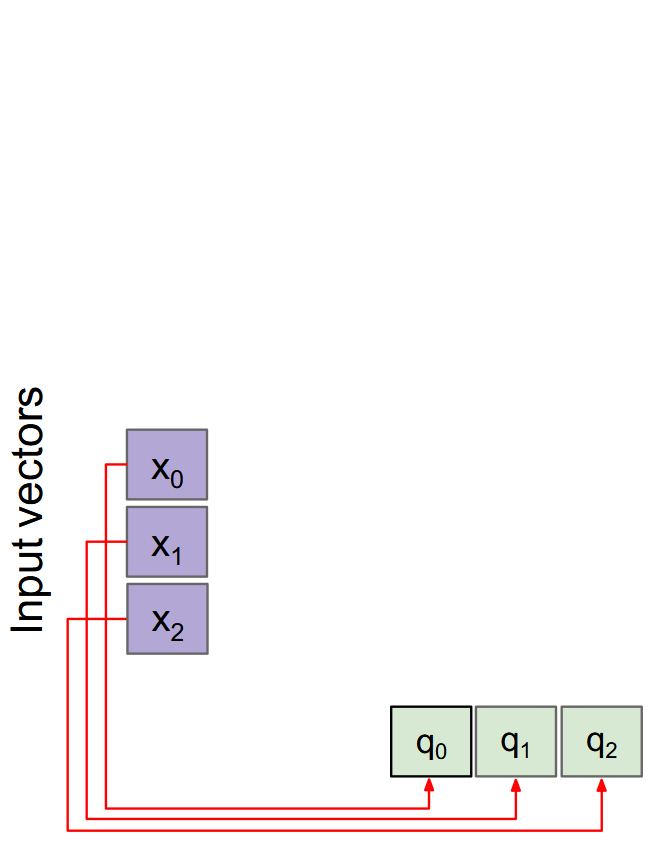
\includegraphics[width=\textwidth]{pic/self-attention-s.png} 
				\vspace{0.5em}
			\end{column}
			
			% Center column: Formulas
			\begin{column}{0.44\textwidth}
%				\textbf{Outputs:} \\
%				Context vectors: $\mathbf{y}$ (\textit{shape: } $D_v$) \\[1em]
				
				\textbf{Operations:}
				\begin{itemize}
					\item Key vectors: $\mathbf{k} = W_k^T \mathbf{x}$
					\item Value vectors: $\mathbf{v} = W_v^T \mathbf{x}$
					\item \textcolor{blue}{Query vectors: $\mathbf{q} = W_q^T \mathbf{x}$}
					\item \textbf{Alignment}: $e_{i,j} = \frac{\mathbf{q}_j \cdot \mathbf{k}_i}{\sqrt{D_k}}$
					\item \textbf{Attention}: $\mathbf{a} = \texttt{softmax}(\mathbf{e})$
					\item Output: $y_j = \sum_i a_{i,j} \mathbf{v}_i$
				\end{itemize}
				
				\textbf{Inputs:}
				\begin{itemize}
					\item Input vectors: $\mathbf{x}$ (\textit{shape: } $N \times D$)
					\item \st{Queries: $\mathbf{q}$ (\textit{shape: } $M \times D_k$)}
				\end{itemize}
			\end{column}
			
			% Right column: Notes
			\begin{column}{0.35\textwidth}
				\begin{itemize}
					\item We can calculate the query vectors from the input vectors, therefore defining a \textbf{“self-attention”} layer.
					\item Instead, query vectors are calculated using a Fully Connected (FC) layer.
					\item \textbf{No input query vectors anymore.}
				\end{itemize}
				
			\end{column}
		\end{columns}
\vspace{3pt}
\vfill
\begin{tikzpicture}[remember picture,overlay]
	\node[anchor=south west, xshift=0.15cm, yshift=0.22cm] at (current page.south west) {
		\tiny Figure adapted from Fei-Fei Li, Jiajun Wu, and Ruohan Gao Lecture Slides, Stanford University
	};
\end{tikzpicture}
\end{frame}

\begin{frame}{Self-Attention Layer}
	\begin{columns}
		% Left column: Image
		\begin{column}{0.35\textwidth}
			\centering
			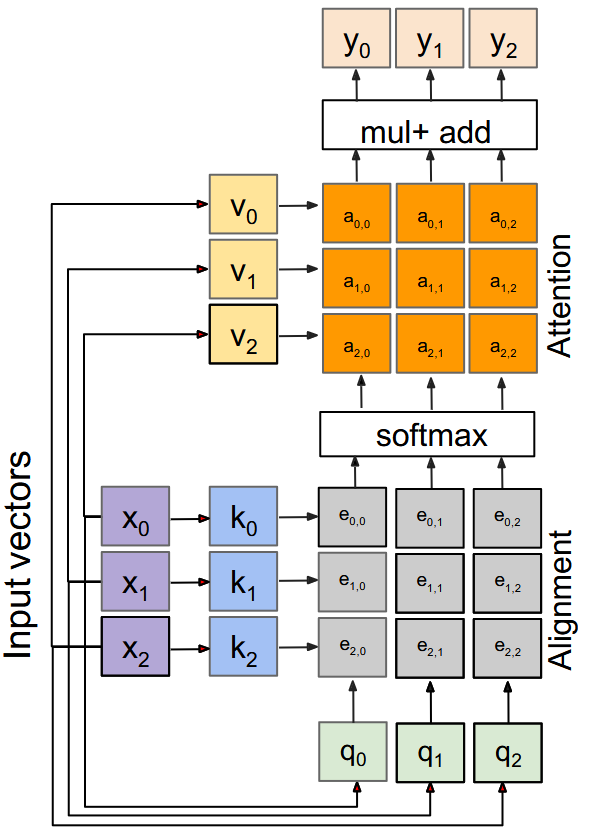
\includegraphics[width=\textwidth]{pic/self-attention-s-1.png} 
			\vspace{0.5em}
		\end{column}
		
		% Center column: Formulas
		\begin{column}{0.58\textwidth}
			\textbf{Outputs:} \\
			Context vectors: $\mathbf{y}$ (\textit{shape: } $D_v$) \\[1em]
			
			\textbf{Operations:}
			\begin{itemize}
				\item Key vectors: $\mathbf{k} = W_k^T \mathbf{x}$
				\item Value vectors: $\mathbf{v} = W_v^T \mathbf{x}$
				\item \textcolor{blue}{Query vectors: $\mathbf{q} = W_q^T \mathbf{x}$}
				\item \textbf{Alignment}: $e_{i,j} = \frac{\mathbf{q}_j \cdot \mathbf{k}_i}{\sqrt{D_k}}$
				\item \textbf{Attention}: $\mathbf{a} = \texttt{softmax}(\mathbf{e})$
				\item Output: $y_j = \sum_i a_{i,j} \mathbf{v}_i$
			\end{itemize}
			
			\textbf{Inputs:}
			\begin{itemize}
				\item Input vectors: $\mathbf{x}$ (\textit{shape: } $N \times D$)
			\end{itemize}
		\end{column}

	\end{columns}
\vspace{3pt}
\vfill
\begin{tikzpicture}[remember picture,overlay]
	\node[anchor=south west, xshift=0.15cm, yshift=0.22cm] at (current page.south west) {
		\tiny Figure adapted from Fei-Fei Li, Jiajun Wu, and Ruohan Gao Lecture Slides, Stanford University
	};
\end{tikzpicture}
\end{frame}

\begin{frame}{Self-Attention: Core Theorem}
    \textcolor{blue}{\textbf{Self-Attention Properties}}
    \newline
        Self-attention layers can model dependencies between all elements in an input sequence in parallel, capturing long-range relationships efficiently.

    \begin{itemize}
            \item Global connectivity
            \item Parallel computation
            \item Position-independent weighting
            \item $O(n^2)$ complexity for sequence length $n$
    \end{itemize}
\end{frame}

%\begin{frame}{Self-Attention: Mathematical Foundation}
%    \begin{itemize}
%        \item Input sequence: $X = [x_1, x_2, ..., x_n] \in \mathbb{R}^{n \times d}$
%        \item Linear projections:
%        \begin{align*}
%            Q &= XW^Q \in \mathbb{R}^{n \times d_k} \\
%            K &= XW^K \in \mathbb{R}^{n \times d_k} \\
%            V &= XW^V \in \mathbb{R}^{n \times d_v}
%        \end{align*}
%        \item Attention computation:
%        \begin{equation*}
%            \text{Attention}(Q, K, V) = \text{softmax}\left(\frac{QK^T}{\sqrt{d_k}}\right)V
%        \end{equation*}
%    \end{itemize}
%\end{frame}

\begin{frame}{Parallel Processing}
    \begin{itemize}
        \item Matrix multiplication enables parallel computation:
        \begin{equation*}
            S = QK^T = \begin{bmatrix}
            (q_1k_1^T) & \cdots & (q_1k_n^T) \\
            \vdots & \ddots & \vdots \\
            (q_nk_1^T) & \cdots & (q_nk_n^T)
            \end{bmatrix}
        \end{equation*}
        \item All $n^2$ interactions computed simultaneously
        \item No sequential dependencies between computations
    \end{itemize}
    \textcolor{blue}{\textbf{Key Insight}}
    \newline
        Unlike RNNs, there is no need to wait for previous timesteps
\end{frame}

\begin{frame}{Global Dependencies}
    \begin{itemize}
        \item Attention weights between positions $i$ and $j$:
        \begin{equation*}
            \alpha_{ij} = \frac{\exp(q_i^Tk_j/\sqrt{d_k})}{\sum_{l=1}^n \exp(q_i^Tk_l/\sqrt{d_k})}
        \end{equation*}
        \begin{itemize}
            \item Properties:
            \item $\alpha_{ij}$ depends only on compatibility of $i$ and $j$
            \item No distance-based attenuation
            \item Softmax ensures $\sum_j \alpha_{ij} = 1$
        \end{itemize}
    \end{itemize}
\end{frame}

%\begin{frame}{Global Dependencies}
%        \begin{figure}
%        \centering
%        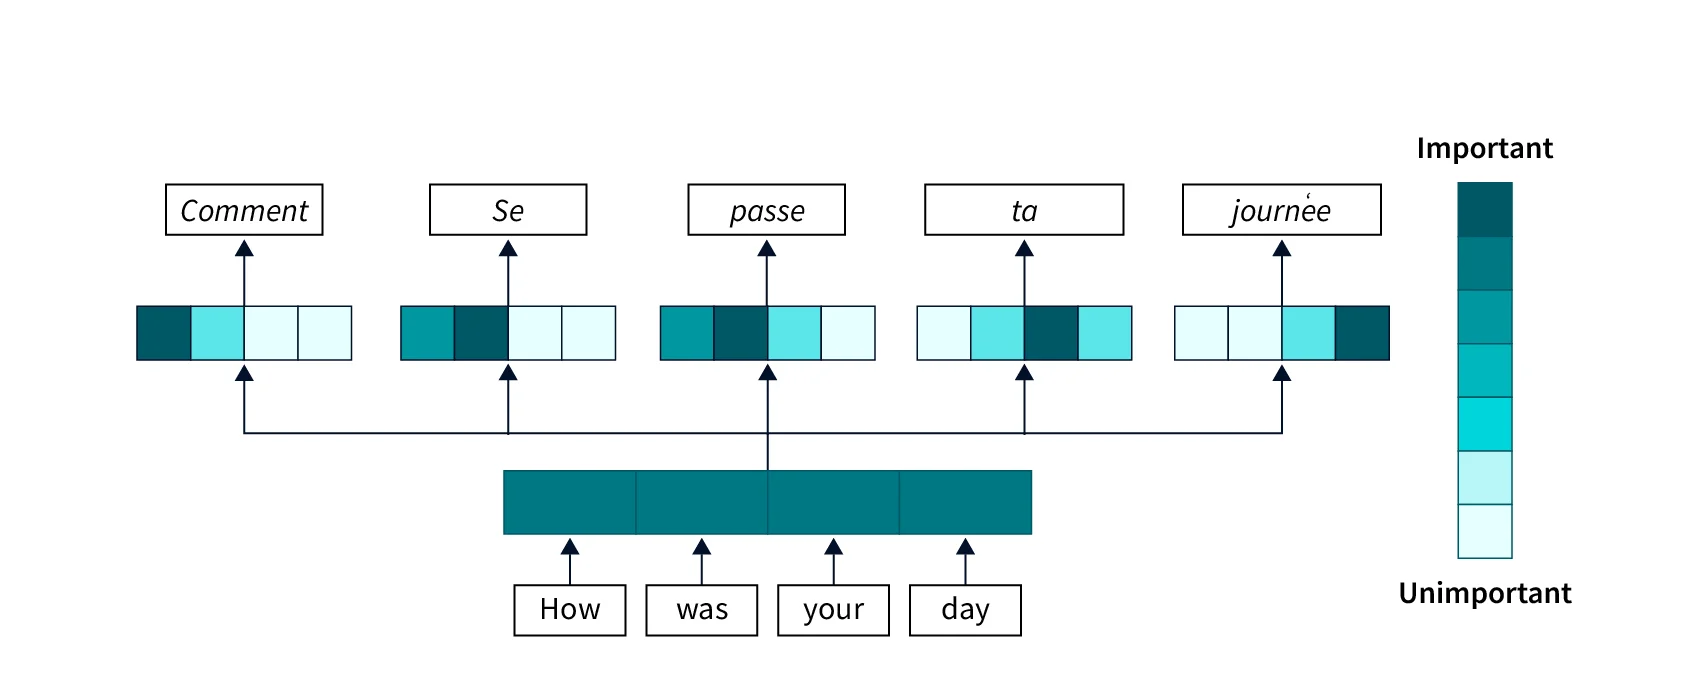
\includegraphics[width=0.85\textwidth]{pic/attention-weights.png}
%        %\caption{Attention weight visualization}
%    \end{figure}
%\vspace{7pt}   
%\vfill
%\begin{tikzpicture}[remember picture,overlay]
%	\node[anchor=south west, xshift=0.15cm, yshift=0.22cm] at (current page.south west) {
%		\tiny Figure adapted from Navaneeth Malingan, Attention Mechanism in Deep Learning, Scaler Topics
%	};
%\end{tikzpicture}
%\end{frame}

\begin{frame}{Computational Efficiency}
    \begin{columns}
        \column{0.5\textwidth}
        \textbf{Complexity Analysis}
        \begin{itemize}
            \item Matrix multiplication: $O(n^2d)$
            \item Softmax: $O(n^2)$
            \item Total: $O(n^2d)$
        \end{itemize}
        
        \column{0.5\textwidth}
        \textbf{Optimizations}
        \begin{itemize}
            \item Sparse attention
            \item Linear attention
            \item Sliding window
        \end{itemize}
    \end{columns}

    \vspace{0.5cm}
    \textcolor{blue}{\textbf{Memory-Computation Tradeoff}}
    
    \vspace{0.2cm}
    More memory than RNNs ($O(n)$), but enables parallelization.
    
\end{frame}

\begin{frame}{Implementation Details}
    \begin{itemize}
        \item Practical considerations:
        \begin{itemize}
            \item Scale factor $\sqrt{d_k}$ prevents vanishing gradients
            \item Mask for causal attention (decoder)
            \item Dropout for regularization
        \end{itemize}
    \end{itemize}
    \begin{equation*}
        \text{MaskedAttention}(Q, K, V) = \text{softmax}\left(\frac{QK^T}{\sqrt{d_k}} + M\right)V
    \end{equation*}
    where $M_{ij} = -\infty$ for masked positions
\end{frame}

\begin{frame}{Self Attention}
        Self-attention satisfies all claimed properties:
        \begin{enumerate}
            \item Parallel computation: Matrix operations
            \item Global dependencies: Direct pairwise attention
            \item Efficient computation: $O(n^2d)$ complexity
            \item Learnable patterns: Attention weights
        \end{enumerate}
    \textcolor{blue}{\textbf{Important Note}}
    \newline
        These properties make self-attention particularly suitable for:
        \begin{itemize}
            \item Natural language processing
            \item Graph neural networks
            \item Computer vision (with modifications)
        \end{itemize}
\end{frame}

\section{Types of Attention}
\begin{frame}{Self-Attention vs Cross-Attention}
	\begin{columns}
		\column{0.5\textwidth}
		\textbf{Self-Attention}
		\begin{itemize}
			\item Queries, Keys, and Values are derived from the same sequence.
			\item Each position attends to all other positions in the sequence.
		\end{itemize}
		\vspace{0.5em}
		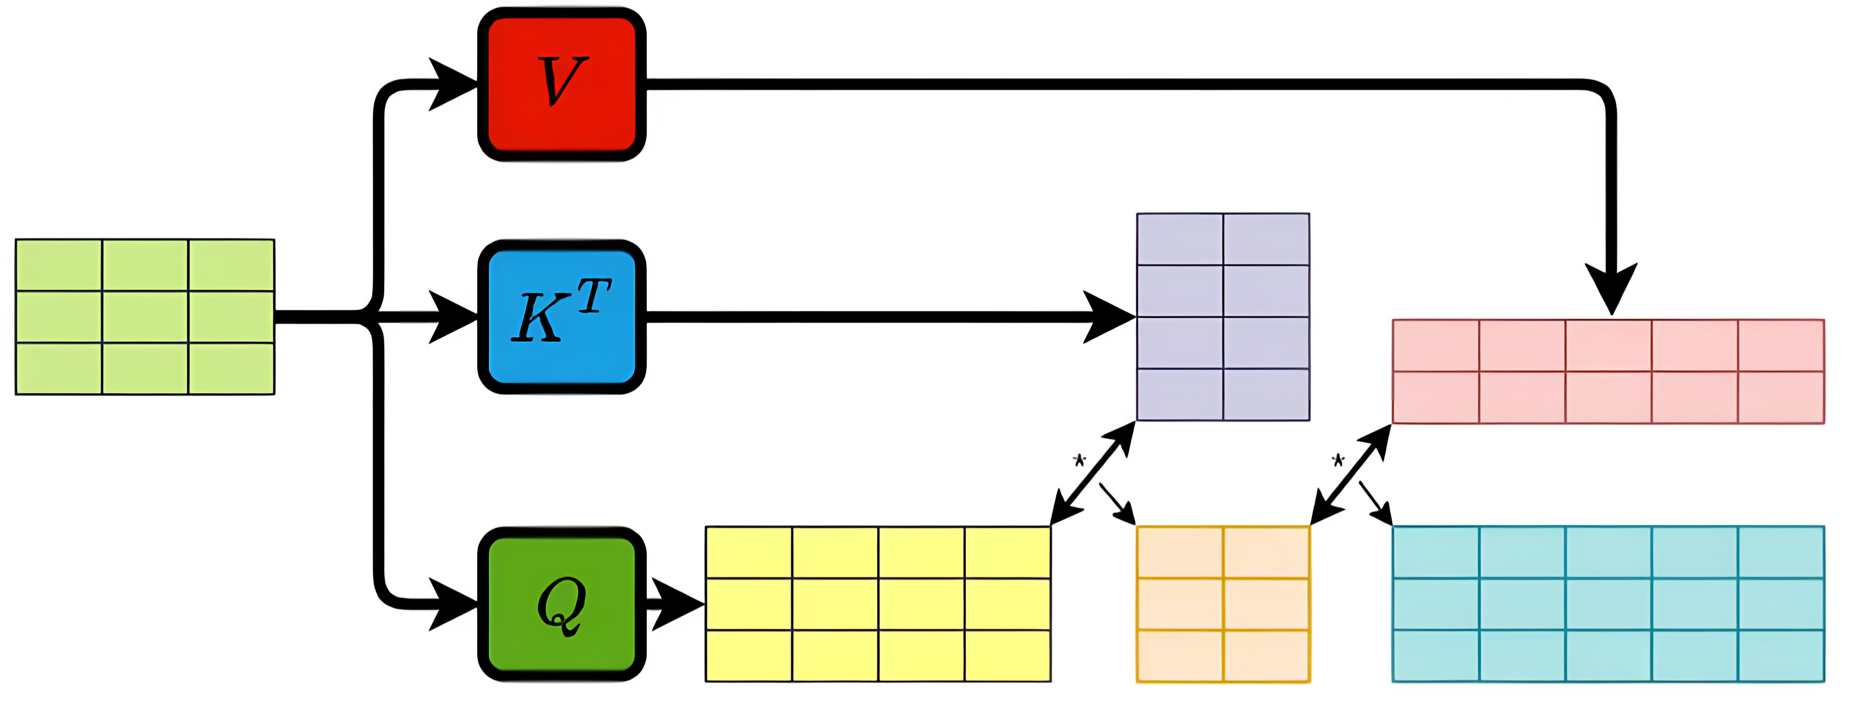
\includegraphics[width=\textwidth]{pic/self-attention.png}
		
		\column{0.5\textwidth}
		\textbf{Cross-Attention}
		\begin{itemize}
			\item Queries come from one sequence.
			\item Keys and Values come from another sequence.
		\end{itemize}
		\vspace{0.5em}
		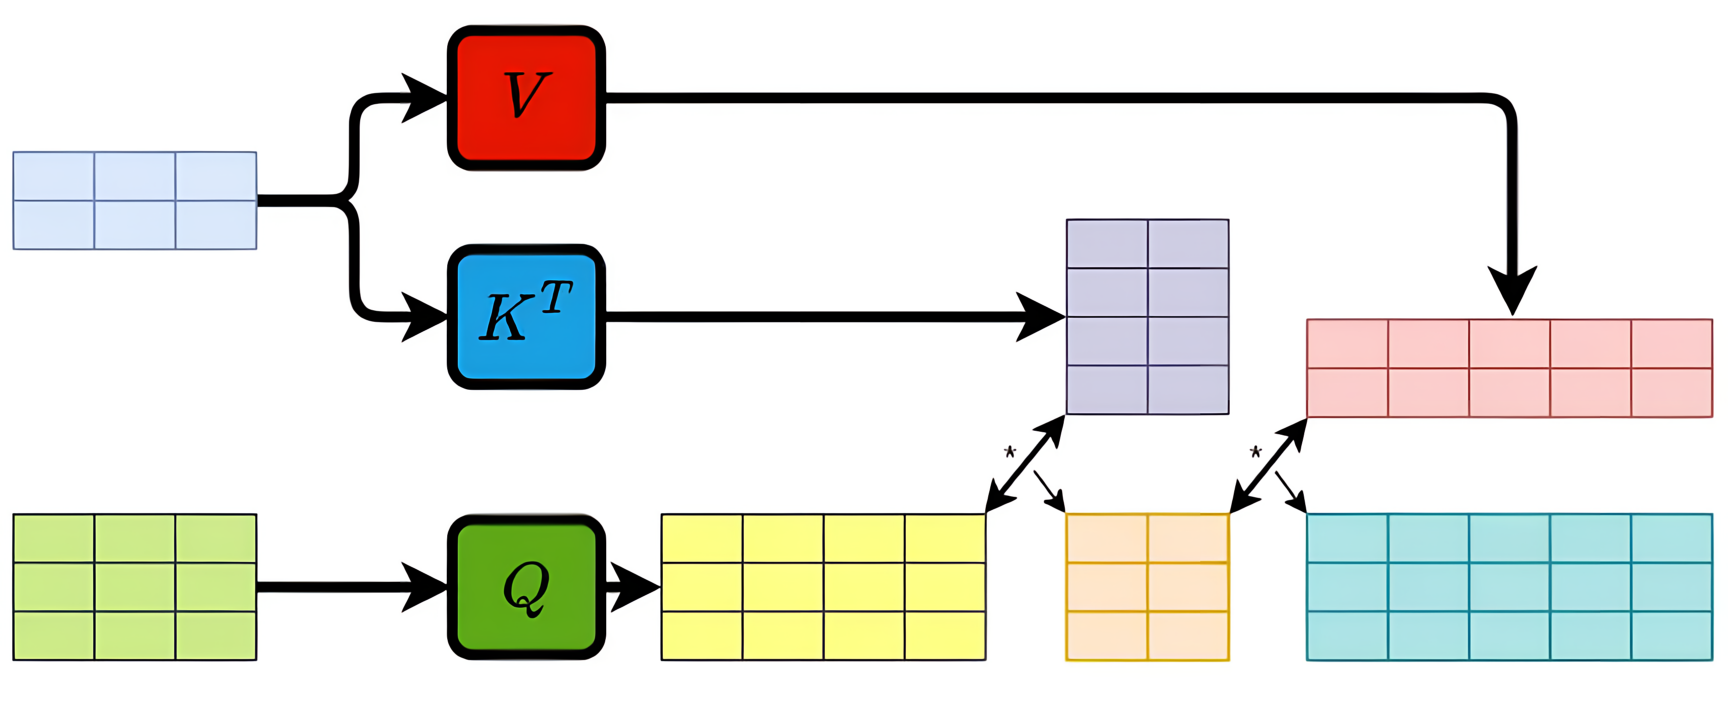
\includegraphics[width=\textwidth]{pic/cross-attention.png}
	\end{columns}
\vspace{5pt}
\vfill
\begin{tikzpicture}[remember picture,overlay]
	\node[anchor=south west, xshift=0.15cm, yshift=0.22cm] at (current page.south west) {
		\tiny Figure adapted from Soran Ghaderi, Transformers-in-action-attention-is-all-you-need, TowardsDataScience blog
	};
\end{tikzpicture}
\end{frame}

\begin{frame}{Self-Attention vs RNN}
	
	%	\begin{figure}
		%		\centering
		%		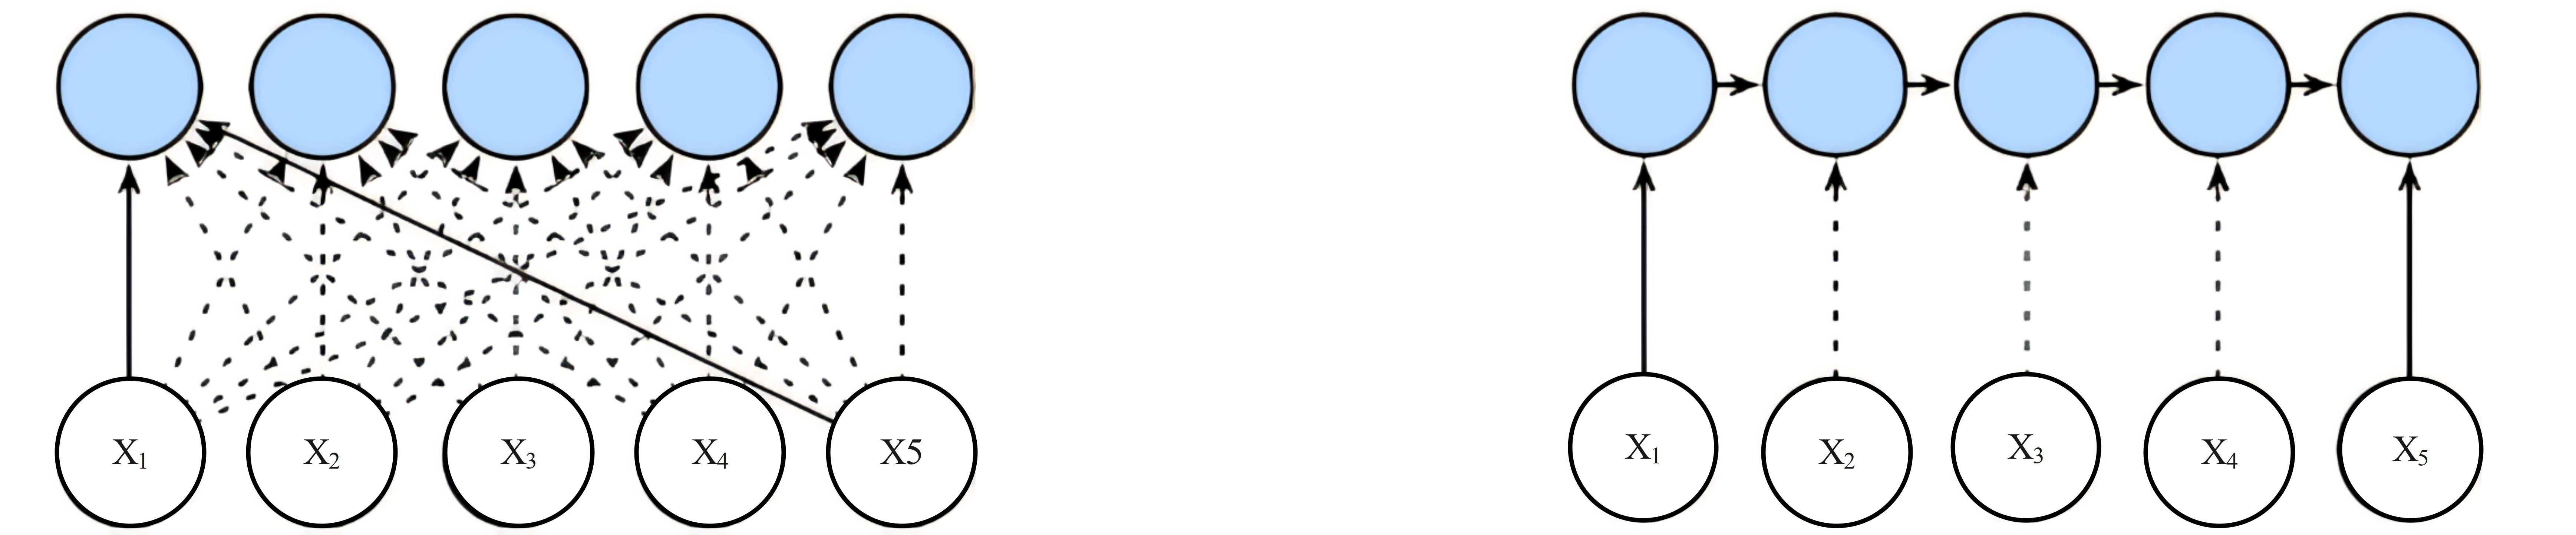
\includegraphics[width=0.95\textwidth]{pic/rnn-self-attention-1.jpg}
		%	\end{figure}
	\begin{columns}
		\column{0.55\textwidth}
		\begin{figure}
			\centering
			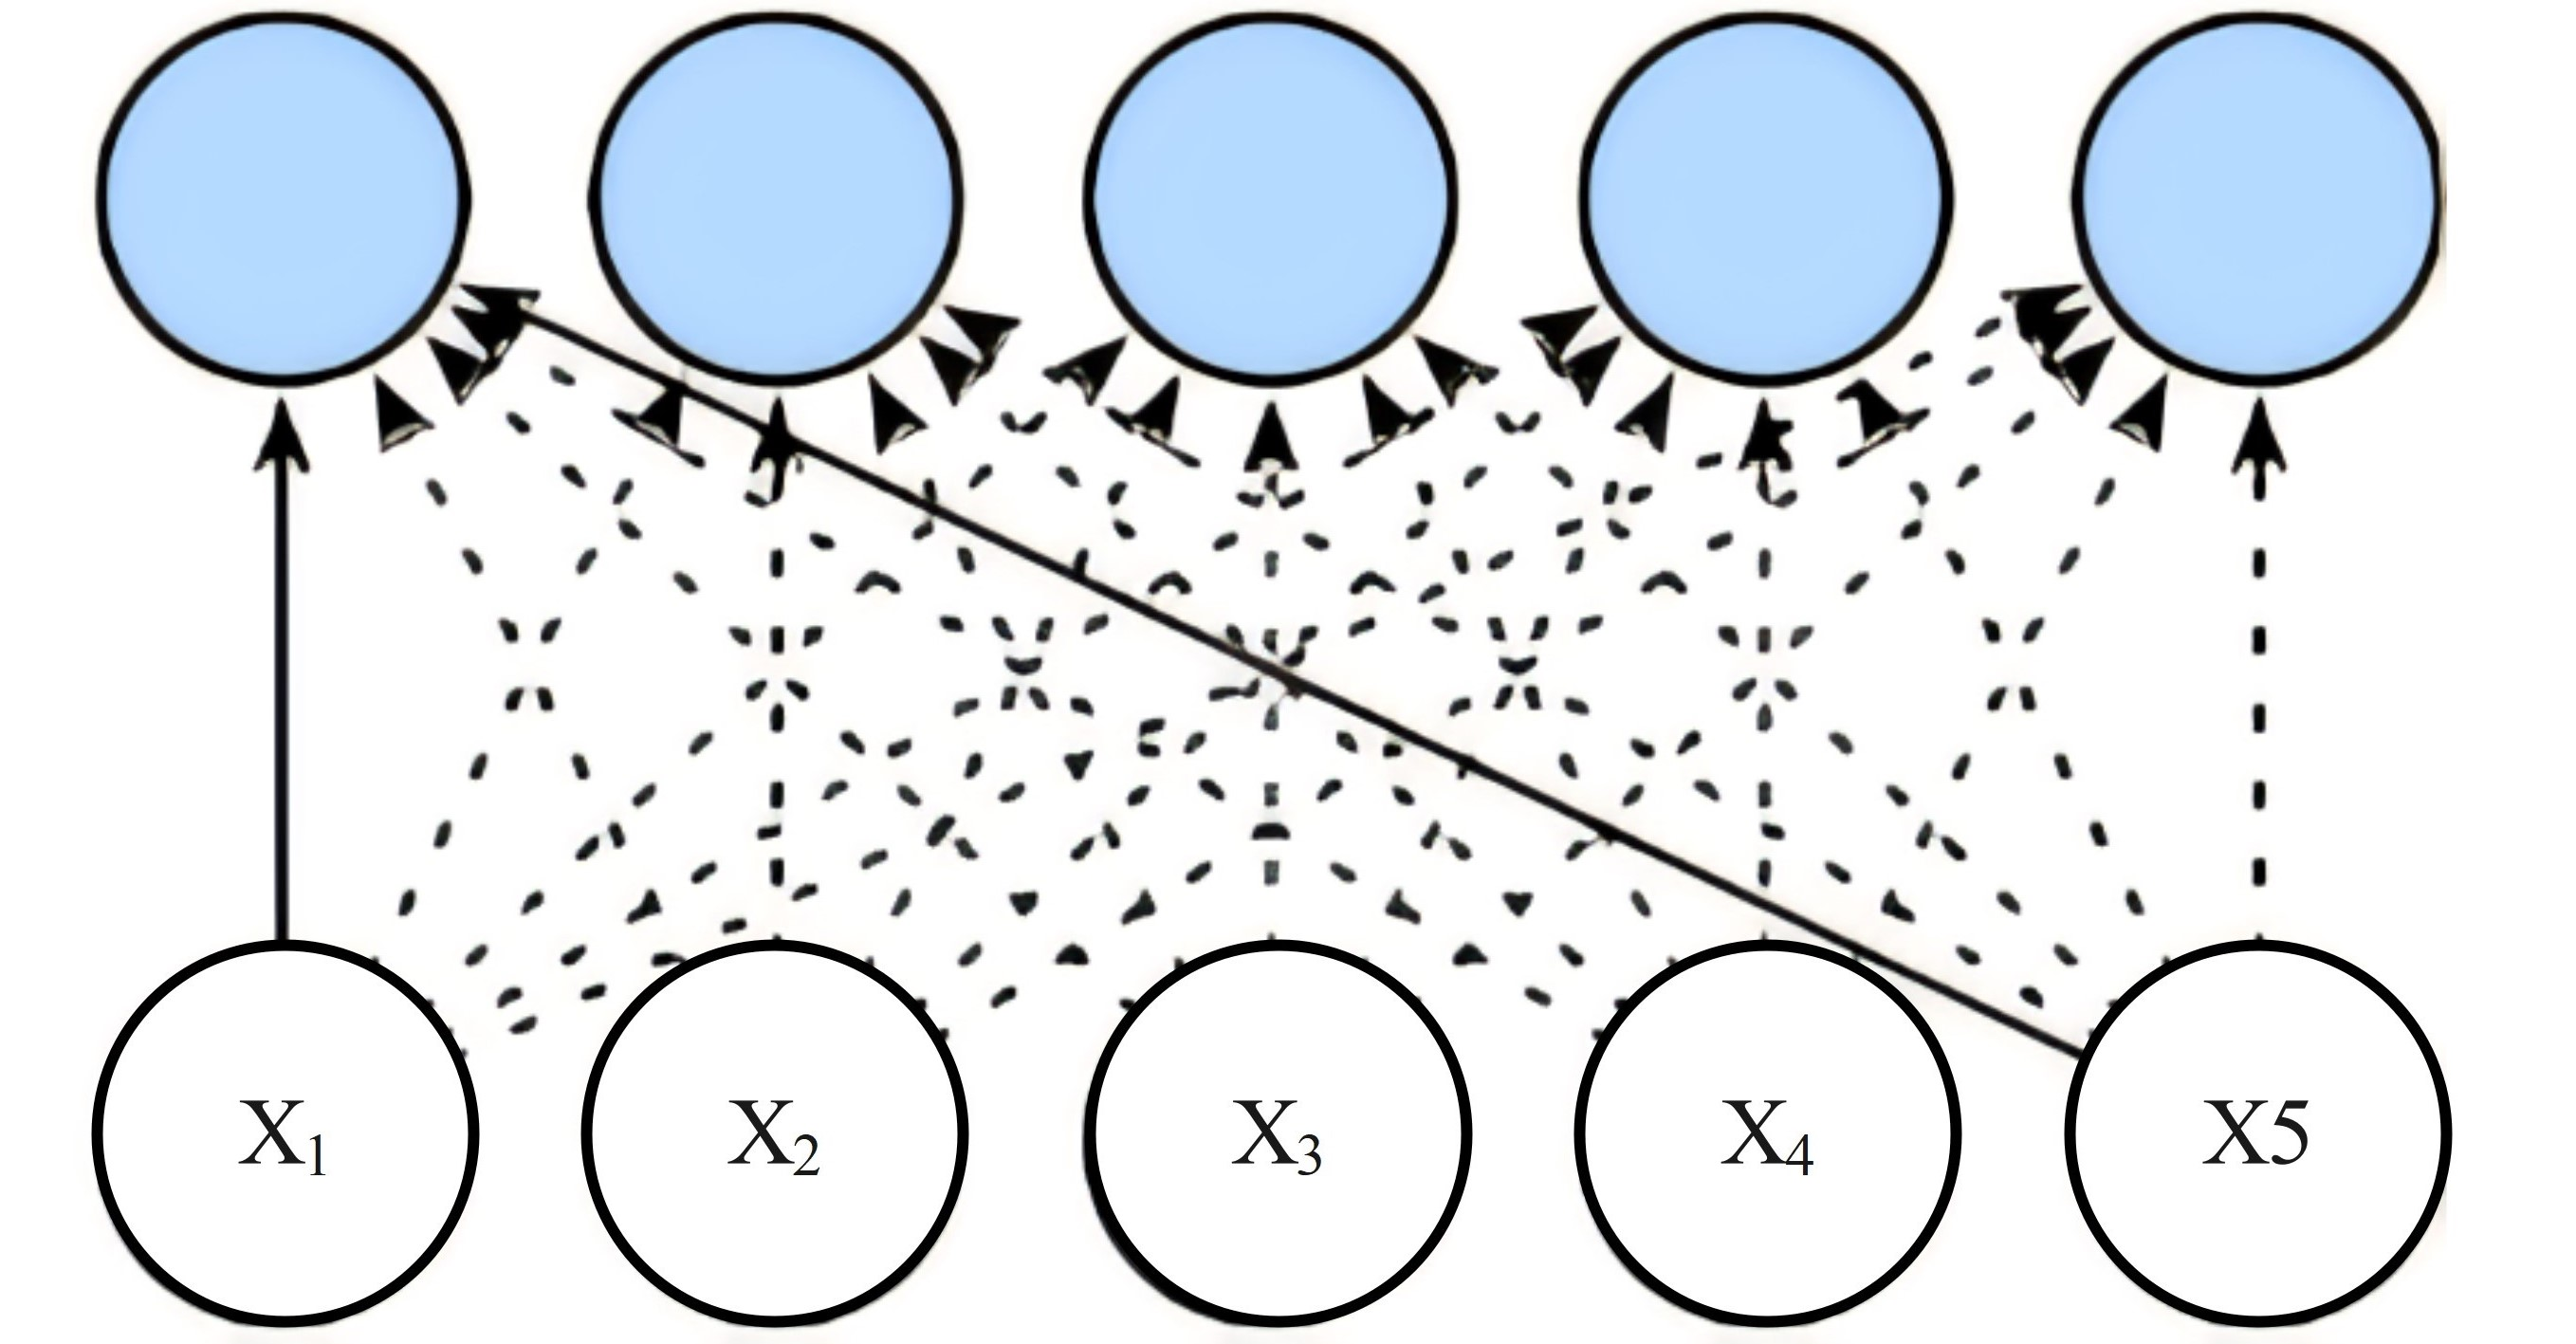
\includegraphics[width=0.7\textwidth]{pic/self-attention--1.jpg}
		\end{figure}
		\textbf{Self-Attention:}
		\begin{itemize}
			\item Directly accesses key information at any position in the input sequence.
			\item Allows the model to \textbf{``attend''} to the most relevant information in the sequence.
			%			\item Avoids compressing all information into a single hidden state.
			%			\item Naturally captures relationships between distant elements in the sequence.
		\end{itemize}
		
		\column{0.52\textwidth}
		\begin{figure}
			\centering
			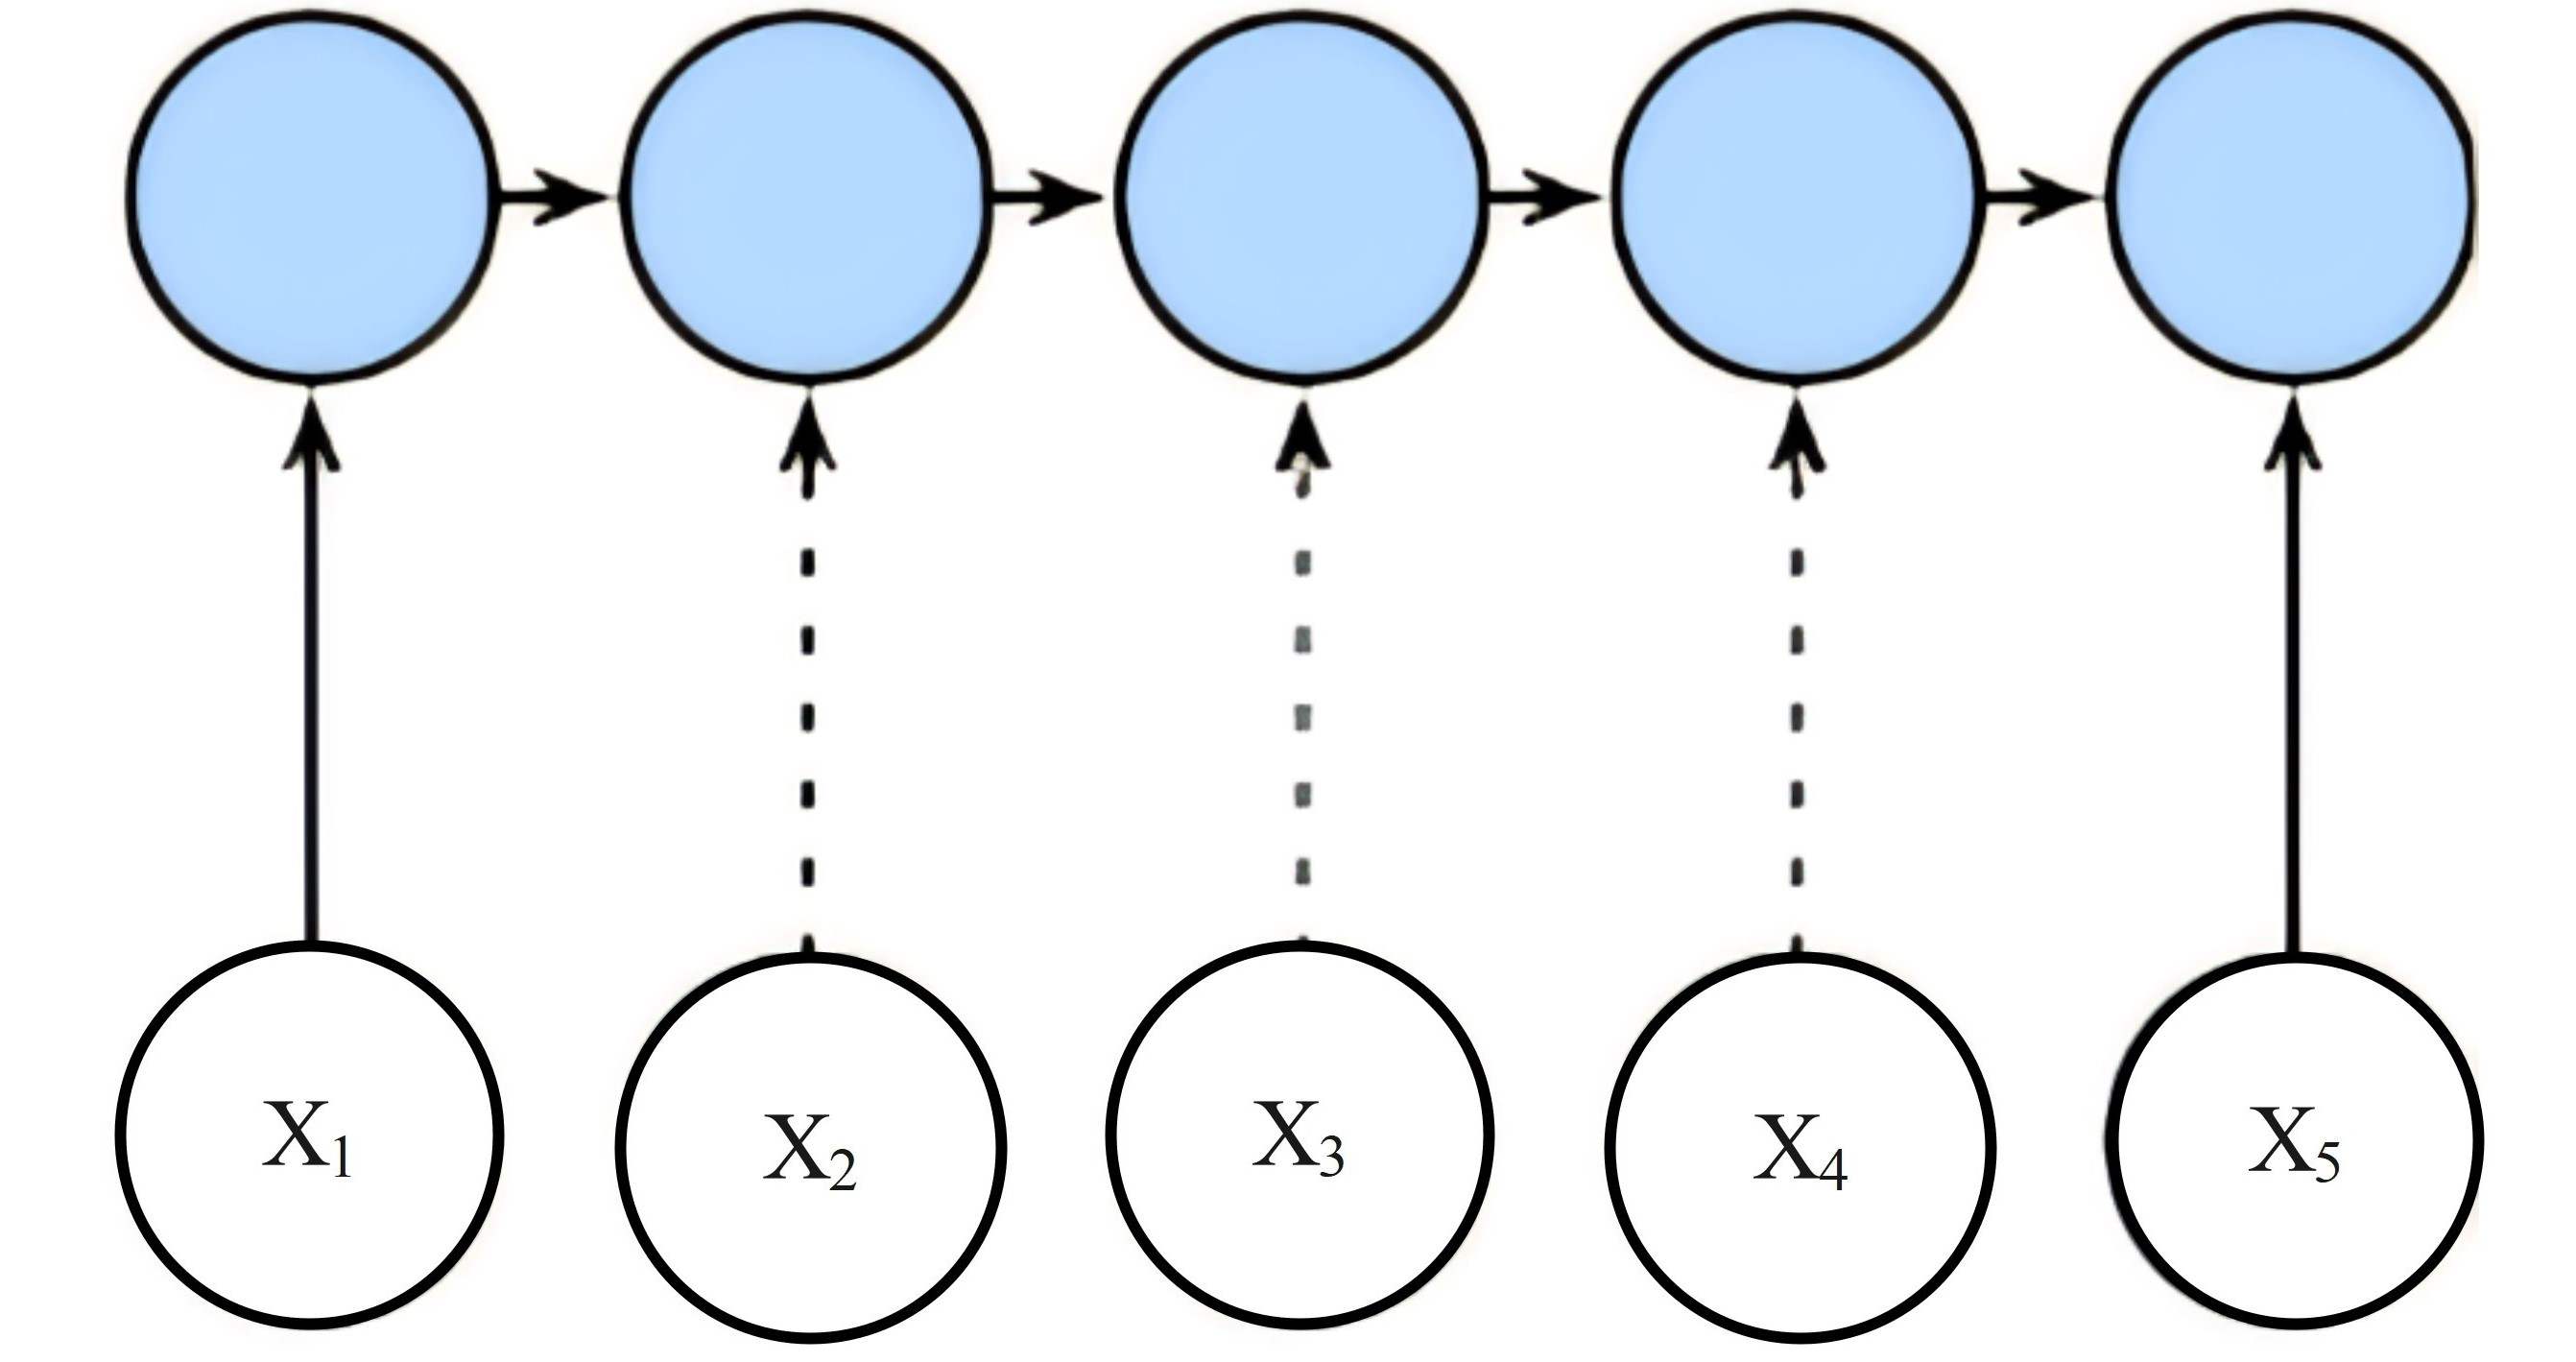
\includegraphics[width=0.72\textwidth]{pic/rnn-1.jpg}
		\end{figure}
		\textbf{RNN:}
		\begin{itemize}
			\item Processes input sequentially, making distant information harder to access.
			\item Relies on the hidden state at the current time step to propagate information.
			%			\item Compresses all information into a single hidden state, which can lead to loss of details.
			%			\item Struggles with capturing relationships between distant elements due to vanishing gradients.
		\end{itemize}
	\end{columns}
	\vspace{6 pt}
	\vfill
	\begin{tikzpicture}[remember picture,overlay]
		\node[anchor=south west, xshift=0.15cm, yshift=0.22cm] at (current page.south west) {
			\tiny Figure adapted from Attention Mechanisms and Transformers D2L.ai Course
		};
	\end{tikzpicture}
\end{frame}

\section{Positional Encoding}

\begin{frame}{Positional Encoding Motivation}
	\begin{itemize}
		\item Unlike RNNs, which process tokens sequentially, self-attention enables parallel computation.
		\item Note that \textbf{self-attention} by itself \textbf{doesn't preserve the order of the sequence}.
		\item What do we do if it really matters that the model knows in which order the input sequence arrived?
	\end{itemize}
\end{frame}

\begin{frame}{Positional Encoding}
    \begin{itemize}
        \item Problem: Self-Attention is position-agnostic
        \item Solution: Add position information to embeddings
        \item Using sinusoidal functions:
    \end{itemize}
		\begin{equation*}
			PE_{(pos, 2i)} = \sin\left(\frac{pos}{10000^{\frac{2i}{d_{model}}}}\right)
		\end{equation*}
		\begin{equation*}
			PE_{(pos, 2i+1)} = \cos\left(\frac{pos}{10000^{\frac{2i}{d_{model}}}}\right)
		\end{equation*}

    \begin{itemize}
	\item \textbf{Definitions:}
	\begin{itemize}
		\item \( \texttt{pos} \): The position of a word in the input sequence.
		\item \( \texttt{i} \): The index of the feature in the embedding vector.
		\item \( \texttt{$d_{model}$} \): The dimensionality of the model's embedding space.
	\end{itemize}
\end{itemize}
    
\end{frame}

\begin{frame}{Positional Encoding Dimension Dependency}
	\begin{figure}
		\centering
		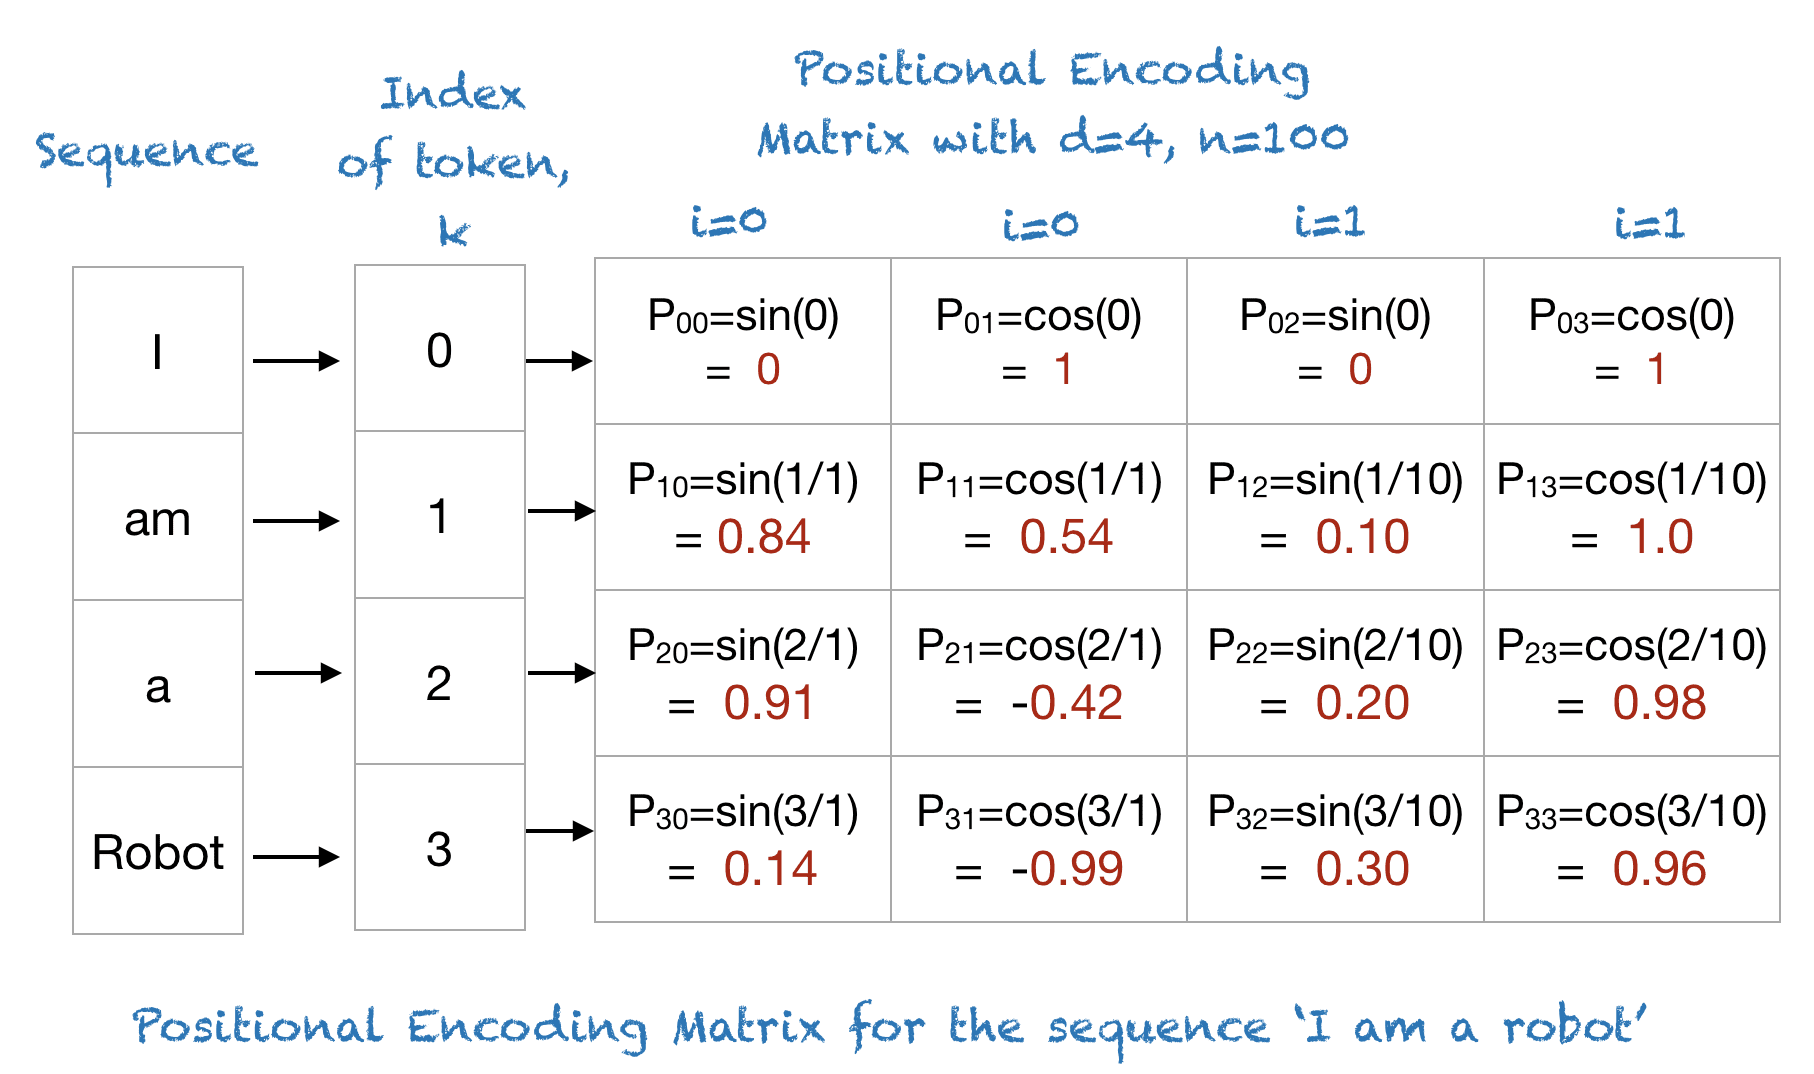
\includegraphics[width=0.77\textwidth]{pic/example.png}
		\label{fig:positional-encoding-1-1-1}
	\end{figure}
	\vspace{5pt}
	\vfill
	\begin{tikzpicture}[remember picture,overlay]
		\node[anchor=south west, xshift=0.15cm, yshift=0.22cm] at (current page.south west) {
			\tiny Figure adapted from Mehreen Saeed, 'A Gentle Introduction to Positional Encoding in Transformer Models,' Machine-Learning Mastery blog
		};
	\end{tikzpicture}
\end{frame}

\begin{frame}{Incorporating Positional Encoding in Self-Attention}
	\begin{itemize}
		\item Since self-attention doesn’t capture order, we need to encode the sequence order in the keys, queries, and values.
		\item Represent each sequence index as a vector \( p_i \in \mathbb{R}^d \), for \( i \in \{1, 2, \dots, T\} \) (position vectors).
		\item Don’t worry about the composition of \( p_i \) just yet!
		\item Easily incorporate this into self-attention by adding \( p_i \) to our inputs:
		\begin{equation*}
			\mathbf{v}_i = \mathbf{v}_i' + p_i, \quad \mathbf{q}_i = \mathbf{q}_i' + p_i, \quad \mathbf{k}_i = \mathbf{k}_i' + p_i
		\end{equation*}
	\end{itemize}
\end{frame}

%\begin{frame}{Positional Encoding}
%
%    \begin{figure}
%        \centering
%        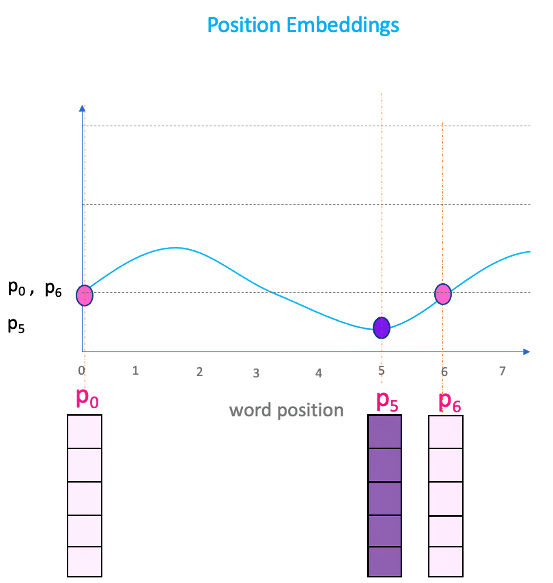
\includegraphics[width=0.47\textwidth]{pic/positional-encoding-1.png}
%        \label{fig:positional-encoding-1}
%    \end{figure}
%\end{frame}

\begin{frame}{Positional Encoding Dimension Dependency}
	\begin{itemize}
			\item The effect of \( d_{model} \) on positional encoding can be seen in the following image.
			\item In the provided image:
				\begin{itemize}
					\item The period of the first two indexes remains constant as \( d_{model} \) changes.
					\item For indexes beyond the first two, the period expands as \( d_{model} \) decreases.
				\end{itemize}
		
	\end{itemize}
	\vspace{-5pt}
	\begin{figure}
		\centering
		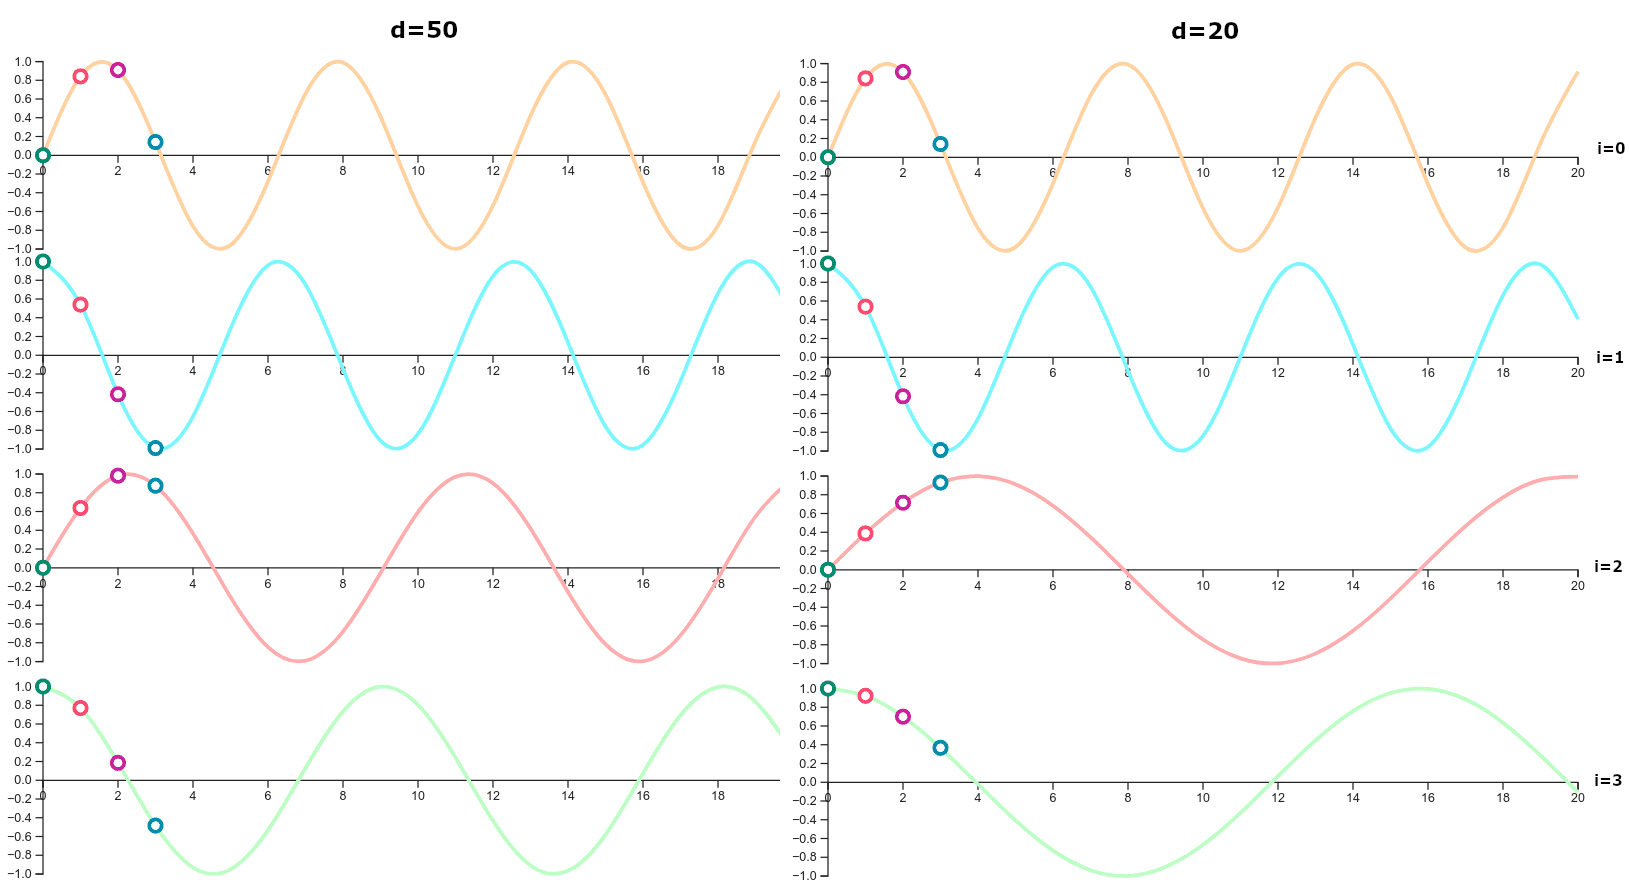
\includegraphics[width=0.63\textwidth]{pic/dimension-comparision.png}
		\label{fig:positional-encoding-1-1-2}
	\end{figure}
	\vspace{5pt}
	\vfill
\begin{tikzpicture}[remember picture,overlay]
	\node[anchor=south west, xshift=0.15cm, yshift=0.22cm] at (current page.south west) {
		\tiny Figure adapted from Kemal Erdem, Understanding Positional Encoding in Transformers, erdem.pl blog
	};
\end{tikzpicture}
\end{frame}

\begin{frame}{Positional Encoding}
	\begin{figure}
		\centering
		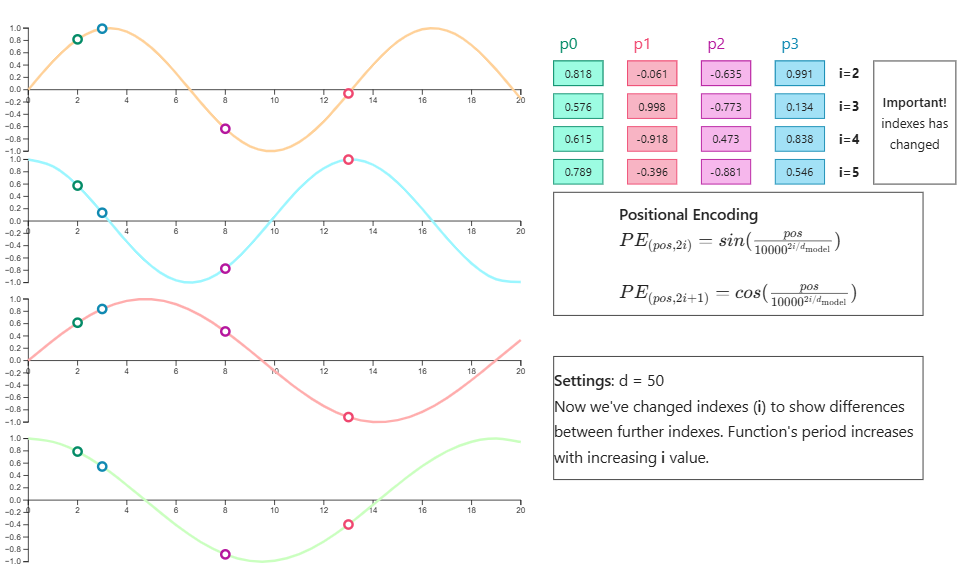
\includegraphics[width=0.77\textwidth]{pic/positional-encoding--s--1.png}
		\label{fig:positional-encoding-1-1-3}
	\end{figure}
	\vspace{5pt}
	\vfill
	\begin{tikzpicture}[remember picture,overlay]
		\node[anchor=south west, xshift=0.15cm, yshift=0.22cm] at (current page.south west) {
			\tiny Figure adapted from Kemal Erdem, Understanding Positional Encoding in Transformers, erdem.pl blog
		};
	\end{tikzpicture}
\end{frame}

\begin{frame}{Positional Encoding}
	\begin{figure}
		\centering
		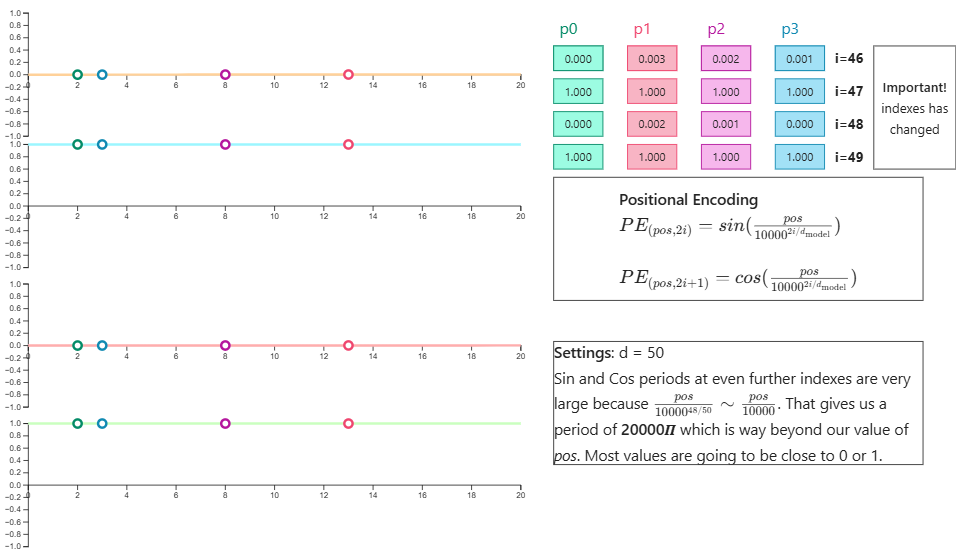
\includegraphics[width=0.75\textwidth]{pic/positional-encoding--s--2.png}
		\label{fig:positional-encoding-1-1-4}
	\end{figure}
	\vspace{5pt}
	\vfill
	\begin{tikzpicture}[remember picture,overlay]
		\node[anchor=south west, xshift=0.15cm, yshift=0.22cm] at (current page.south west) {
			\tiny Figure adapted from Kemal Erdem, Understanding Positional Encoding in Transformers, erdem.pl blog
		};
	\end{tikzpicture}
\end{frame}

\begin{frame}{Positional Encoding}
	\begin{itemize}
		\item Allows the model to learn relative positions.
		\item Works for sequences of any length.
	\end{itemize}
\end{frame}

\section{Multi-Head Attention}

\begin{frame}{Multi-Head Attention}
	
%	\begin{figure}
%		\centering
%		% Left image
%		\begin{minipage}{0.5\textwidth}
%			\centering
%			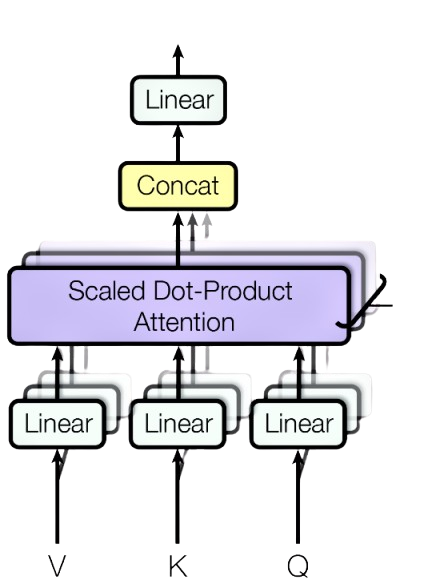
\includegraphics[width=0.9\textwidth]{pic/multihead-attention-2.png}
%			\label{fig:image1-1}
%		\end{minipage}
%		\hfill
%		% Right image
%		\begin{minipage}{0.5\textwidth}
%			\centering
%			
\includegraphics[width=0.9\textwidth]{pic/multihead-dragon.png}
%			\label{fig:image2-2}
%		\end{minipage}
%	\end{figure}
	
	
	    \begin{columns}[c]
		% Left column
		\column{0.5\textwidth}
		\centering
		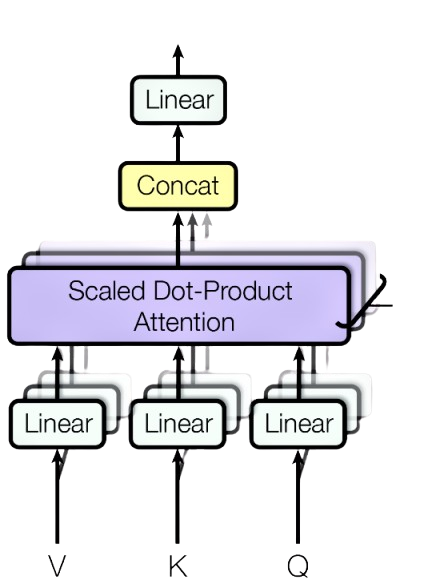
\includegraphics[width=0.7\textwidth]{pic/multihead-attention-2.png}
		
		% Right column
		\column{0.45\textwidth}
		\centering
		
\includegraphics[width=0.85\textwidth]{pic/multihead-dragon.png}
	\end{columns}
	
	\vspace{2pt}
	
	\vfill
	\begin{tikzpicture}[remember picture,overlay]
		\node[anchor=south west, xshift=0.15cm, yshift=0.22cm] at (current page.south west) {
			\tiny Figure adapted from Ashish Vaswani et al. Attention is All You Need paper | Kucedra : The 7 headed dragon, MythLok 
		};
	\end{tikzpicture}
\end{frame}

\begin{frame}{Multi-Head Attention}
    \begin{itemize}
        \item Instead of single attention, use multiple heads
        \item Each head can focus on different aspects
        \item Process in parallel and concatenate
    \end{itemize}
    \begin{equation*}
        \text{MultiHead}(Q,K,V) = \text{Concat}(head_1,\ldots,head_h)W^O
    \end{equation*}
    \begin{equation*}
        head_i = \text{Attention}(QW^Q_i,KW^K_i,VW^V_i)
    \end{equation*}
    
    \begin{figure}
    	\centering
    	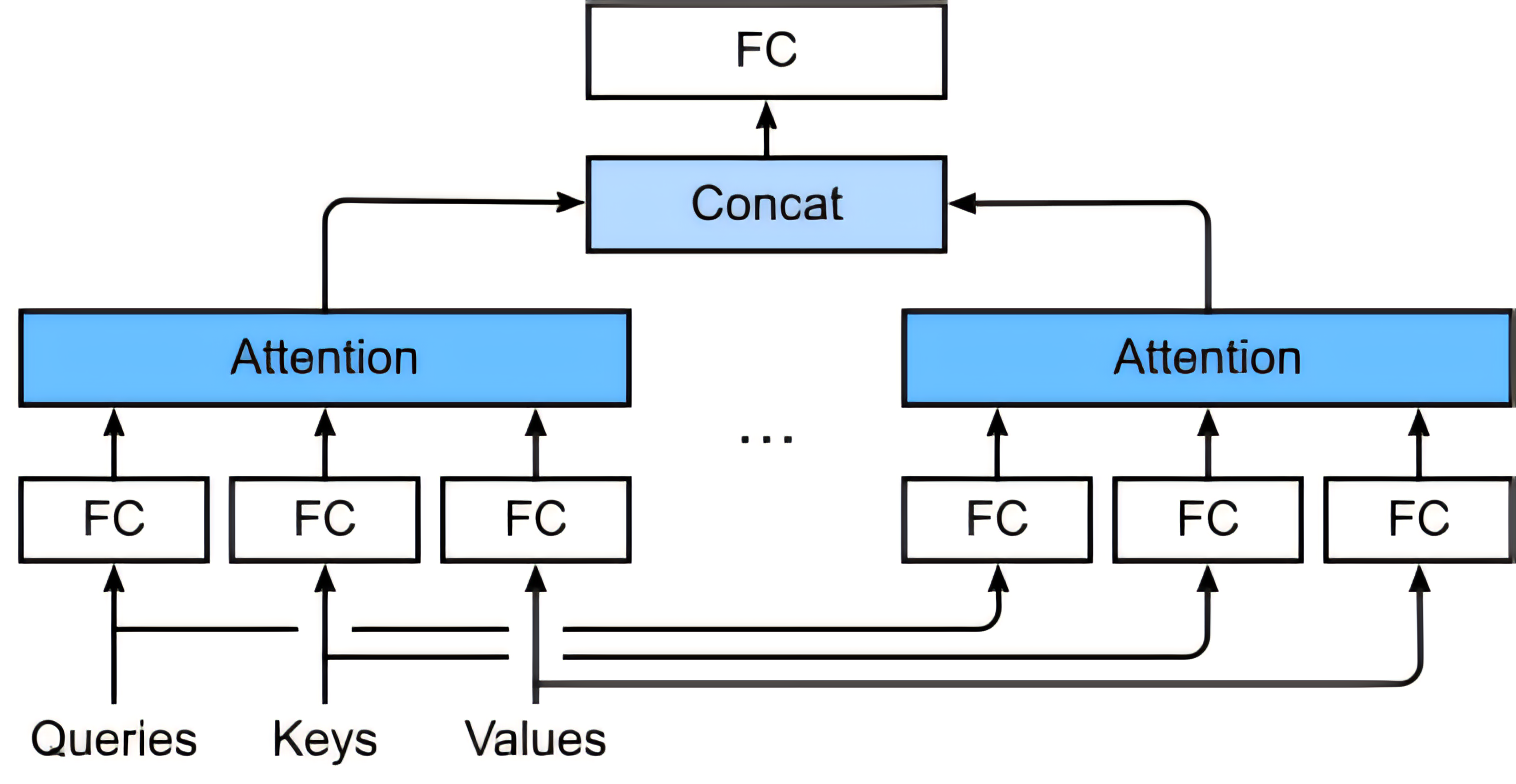
\includegraphics[width=0.5\textwidth]{pic/multi-head-attention__AIE.png}
    	\label{fig:multihead_attention-3}
    \end{figure}
    \vfill
    \begin{tikzpicture}[remember picture,overlay]
    	\node[anchor=south west, xshift=0.15cm, yshift=0.22cm] at (current page.south west) {
    		\tiny Figure adapted from Attention Mechanisms and Transformers D2L.ai Course
    	};
    \end{tikzpicture}
    
\end{frame}

\begin{frame}{Multi-Head Attention}
	\begin{equation*}
		\text{MultiHead}(Q,K,V) = \text{Concat}(head_1,\ldots,head_h)W^O
	\end{equation*}
	
	\begin{figure}
		\centering
		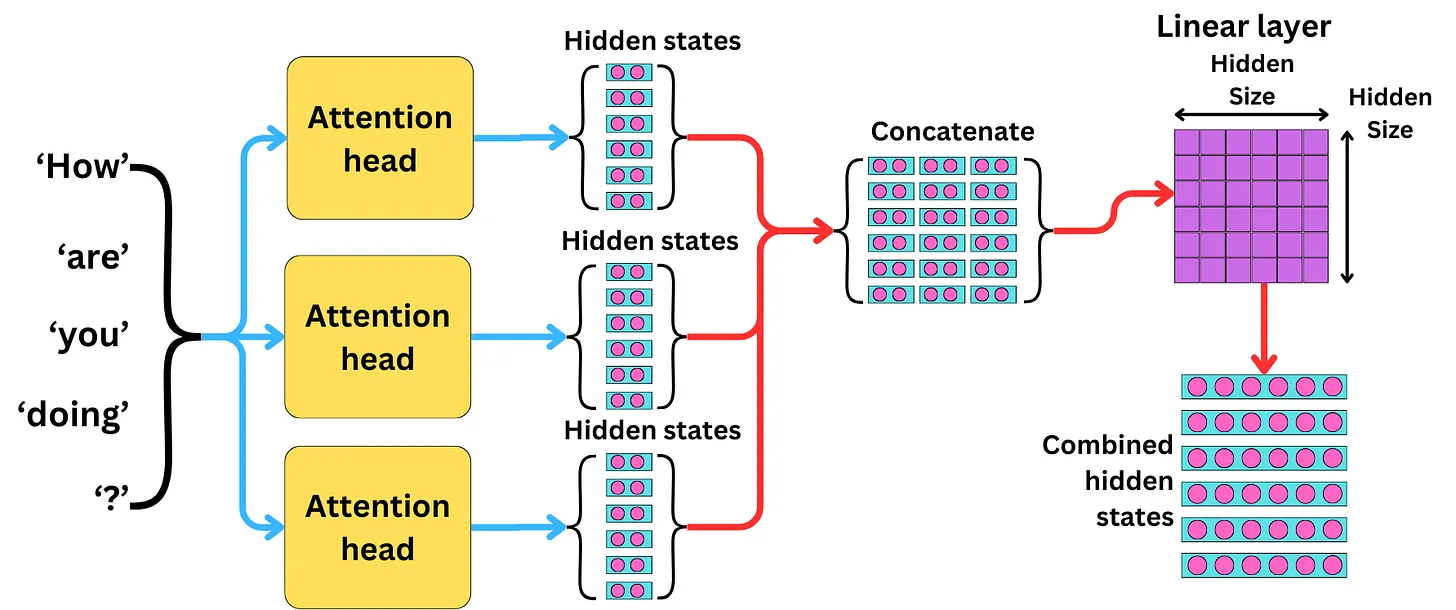
\includegraphics[width=0.7\textwidth]{pic/multihead-attention-in-d-1.png}
		\label{fig:multihead_attention-3-3-3}
	\end{figure}
	\vfill
	\begin{tikzpicture}[remember picture,overlay]
		\node[anchor=south west, xshift=0.15cm, yshift=0.22cm] at (current page.south west) {
			\tiny Figure adapted from Damien Benveniste, 'The Multi-head Attention Mechanism Explained,' The AIEdge Newsletter
		};
	\end{tikzpicture}
	
\end{frame}


\begin{frame}{Multi-Head Attention}
	\begin{equation*}
		head_i = \text{Attention}(QW^Q_i,KW^K_i,VW^V_i)
	\end{equation*}
	
	\begin{figure}
		\centering
		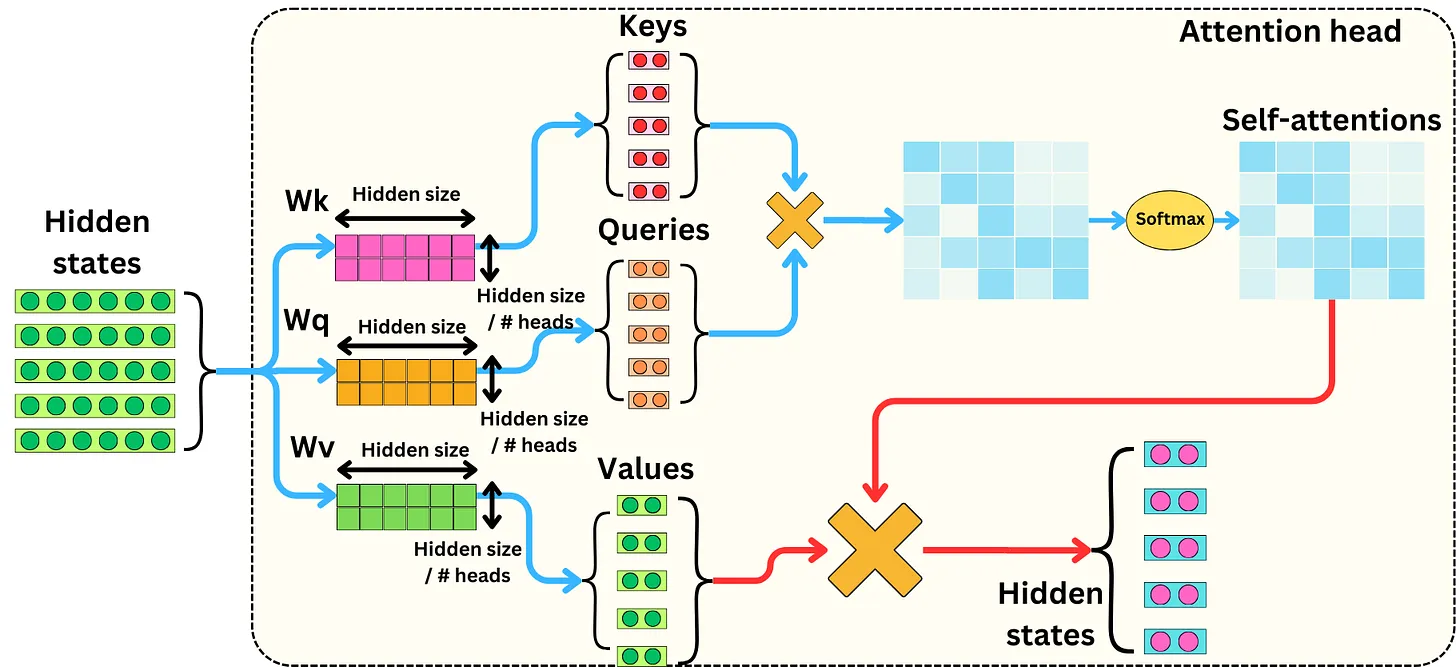
\includegraphics[width=0.7\textwidth]{pic/multihead-attention-in-d-2.png}
		\label{fig:multihead_attention-3-3-4}
	\end{figure}
	\vfill
	\begin{tikzpicture}[remember picture,overlay]
		\node[anchor=south west, xshift=0.15cm, yshift=0.22cm] at (current page.south west) {
			\tiny Figure adapted from Damien Benveniste, 'The Multi-head Attention Mechanism Explained,' The AIEdge Newsletter
		};
	\end{tikzpicture}
	
\end{frame}


\begin{frame}{Multihead Attention Mathematical Formulation}
	\begin{columns}
		\begin{column}{0.5\textwidth}
			\textbf{Attention Head Computation:}
			\begin{equation*}
				head_i = \text{Attention}\left(
				\begin{aligned}
					&QW^Q_i, \\
					&KW^K_i, \\
					&VW^V_i
				\end{aligned}
				\right)
			\end{equation*}
			
			\textbf{Projection Matrices:}
			\begin{itemize}
				\item $W^Q_i \in \mathbb{R}^{d_{model} \times d_k}$
				\item $W^K_i \in \mathbb{R}^{d_{model} \times d_k}$
				\item $W^V_i \in \mathbb{R}^{d_{model} \times d_v}$
			\end{itemize}
		\end{column}
		\begin{column}{0.5\textwidth}
			\textbf{Final Projection:}
			\begin{equation*}
				W^O \in \mathbb{R}^{hd_v \times d_{model}}
			\end{equation*}
			
			\textbf{Definitions:}
			\begin{itemize}
				\item $h$: Number of attention heads
				\item $d_k$: Key/Query dimension
				\item $d_v$: Value dimension
				\item $d_{model}$: Model dimension
			\end{itemize}
		\end{column}
	\end{columns}
\end{frame}

\begin{frame}{Multi-Head Attention}
	
    \begin{columns}
	\column{0.5\textwidth}
	\begin{figure}
		\centering
		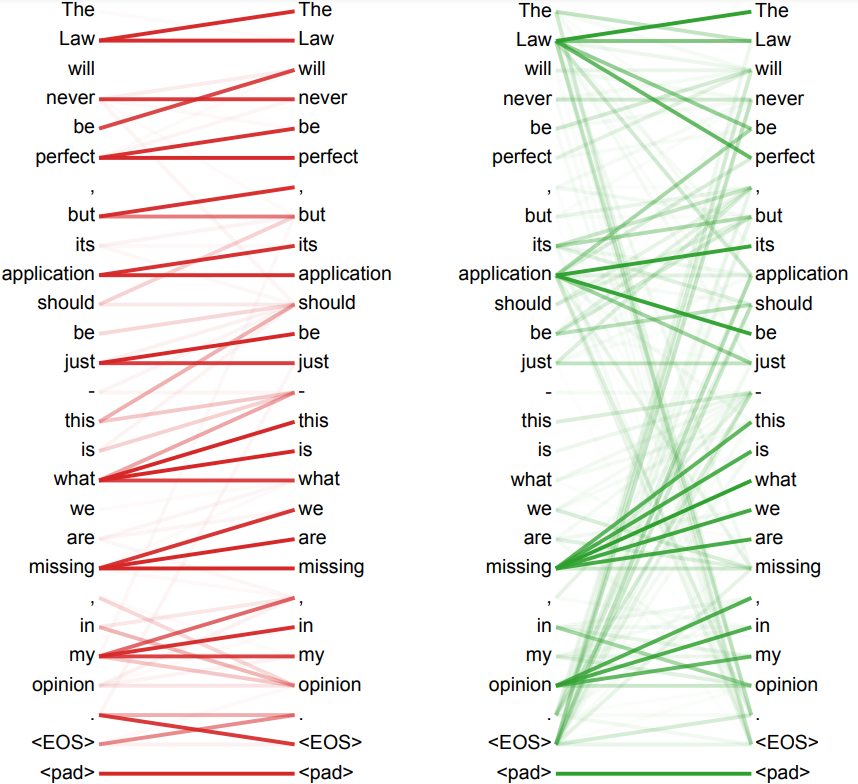
\includegraphics[width=\textwidth]{pic/multihead-attention-s-1.png}
		\label{fig:multihead_attention-1}
	\end{figure}
	

	\column{0.45\textwidth}
    \begin{itemize}
			\item Different attention heads seem to focus on different parts of the sentence.
			\item We show two examples from different heads.
			\item Each head appears to have learned a different task.
			\end{itemize}
\end{columns}

%	\vspace{2pt}
	\vfill
	\begin{tikzpicture}[remember picture,overlay]
		\node[anchor=south west, xshift=0.15cm, yshift=0.22cm] at (current page.south west) {
			\tiny Figure adapted from Ashish Vaswani et al. Attention is All You Need paper
		};
	\end{tikzpicture}
\end{frame}

%\begin{frame}{Multi-Head Attention}
%	
%	\begin{figure}
%		\centering
%		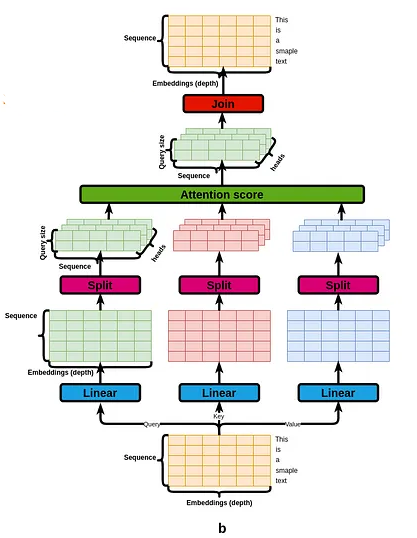
\includegraphics[width=0.38\textwidth]{pic/multihead--1.jpg}
%		\label{fig:multihead_attention-2}
%	\end{figure}
%	\vspace{9pt}
%	\vfill
%	\begin{tikzpicture}[remember picture,overlay]
%		\node[anchor=south west, xshift=0.15cm, yshift=0.22cm] at (current page.south west) {
%			\tiny Figure adapted from Soran Ghaderi, Transformers-in-action-attention-is-all-you-need, TowardsDataScience blog
%		};
%	\end{tikzpicture}
%\end{frame}

\begin{frame}{Multi-Head Attention Benefits}
    \begin{itemize}
        \item Multiple representation subspaces
        \item Can capture different types of relationships like:
        \begin{itemize}
            \item Syntactic dependencies
            \item Semantic relationships
        \end{itemize}
        \item Improves model capacity and stability
    \end{itemize}
    % \begin{figure}
    %     \centering
    %     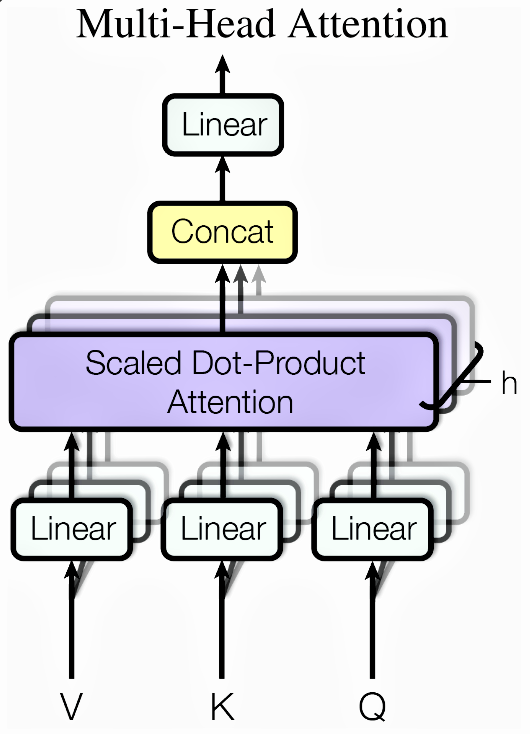
\includegraphics[width=0.7\textwidth]{pic/multihead-attention.png}
    %     \caption{Multi-head attention architecture}
    % \end{figure}
\end{frame}

\begin{frame}{Contributions}
	\textbf{These slides are authored by:}
	\begin{itemize}
		\item Faezeh Sarlakifar
	\end{itemize}
	
\end{frame}


\section{References}

\begin{frame}[allowframebreaks]
    \bibliography{ref}
    \bibliographystyle{ieeetr}
    \nocite{*} % used here because no citation happens in slides
    % if there are too many try use:
    % \tiny\bibliographystyle{alpha}
\end{frame}


\begin{frame}
    \begin{center}
        {\Huge Any Questions?}
    \end{center}
\end{frame}

\end{document}